%!TEX ROOT=formularioFisica.tex

\section{Esercizi}
Questa sezione è dedicata ad alcuni esercizi con relativa risoluzione e spiegazione. Il suo scopo
è quello di chiarire i concetti teorici con esempi pratici.

\subsection*{Consigli}
Ecco alcuni consigli che saranno utili nello svolgimento degli esercizi:
\begin{enumerate}
	\item \textbf{Leggere più volte il problema};
	\item \textbf{Partire dalle formule generali.} Questo aiuterà a imparare le formule e ad 
	applicarle. Leformule particolari sono generalmente derivate e alcune volte anche in casi 
        particolari (alcune variabili pari a zero, masse uguali, \ldots);
	\item \textbf{Guardare corpo per corpo le forze che interagiscono.} Andare per ordine e con calma 
	è una garanzia per evitare di fare errori di calcolo o di teoria. Una volta presa
	questa abitudine, si riduce il numero di errori di distrazione;
	\item \textbf{Avere un sistema unico di risoluzione.} Abituarsi al proprio sistema, seguendo o 
	meno questi consigli, aiuterà ad essere costanti e ad evitare errori di distrazione;
	\item \textbf{Mettere tutti i dati in una "tabella".} Aiuta a visualizzare ciò che si ha e capire
	come ottenere ciò che serve;
	\item \textbf{Scrivere le formule utilizzabili.} Assieme al punto precedente, aiuta ad avere un
	quadro generale di ciò che si va ad affrontare;
	\item \textbf{Ricontrollare i conti a fine di ogni riga.} Nessuno è infallibile, è facile 
	scambiare un segno o fare stupidi errori, ricontrollare scongiura la loro propagazione;
\end{enumerate}

\subsection*{\hyperref[sec:cinematica]{Cinematica}}\label{ex:cinematica}

\subsubsection*{\hyperref[subsec:cinematica:mru]{Moto Rettilineo Uniforme}}\label{ex:mru}
\paragraph{Esercizio 1}
Un poliziotto sta inseguendo un fuggitivo su una strada rettilinea. La velocità del fuggitivo è 
costante a $v_f = 120\,\text{km/h}$ e il poliziotto è a distanza $d=500\,\text{m}$ e ha velocità
pari a $v_p = 180\,\text{km/h}$. Qual è la \textbf{velocità relativa} del poliziotto rispetto al
fuggitivo? Quanto \textbf{tempo} ci vuole perché lo raggiunga?

\divisor

La velocità relativa è molto semplicemente la differenza tra le velocità.
\begin{equation*}
v_r = v_p-v_f \rightarrow v_r = 180-120 = \boxed{60\,\text{km/h}}
\end{equation*}

Per trovare quando i due individui si incontrano basta mettere a sistema le loro due equazioni
della posizione
\begin{equation*}
\begin{cases}
x = x_0 + v_ft\\x = v_pt
\end{cases}\rightarrow
180t = 120t + 500 \rightarrow t = \frac{50}{6} = \boxed{8.3\,\text{s}}
\end{equation*}

\subsubsection*{\hyperref[subsec:cinematica:mrua]{Moto Rettilineo Uniformemente Accelerato}}
\label{ex:mrua}

\paragraph{Esercizio 1}
Un corpo cade liberamente fino a terra che si trova ad una distanza $h$. Sapendo che nell'ultimo 
secondo di volo percorre una distanza pari a $\dfrac{h}{2}$, \textbf{quanto vale $h$}?

\divisor

Dalla formula del MRUA $v^2 = v_0^2 + 2ay$, possiamo sostituire le informazioni che abbiamo per per
trovare la velocità quando il corpo si trova a $\dfrac{h}{2}$
\begin{equation*}
v^2 = v_0^2 + 2ay \rightarrow v = \sqrt{gh}
\end{equation*}
Inserendo ora la velocità nell'equazione oraria possiamo ricavare $h$
\begin{equation*}
y = y_0 + v_0t + \frac{1}{2}gt^2 \rightarrow y = \sqrt{gh} + \frac{1}{2}gt^2
\end{equation*}
e ora non resta che sostituire i dati
\begin{align*}
\frac{h}{2} &= \sqrt{9.81\cdot h} + 9.81 \rightarrow h = 2\sqrt{9.81\cdot h} + 9.81\\
(h-9.81)^2 &= 39.24h \rightarrow h^2 -58.86h + 96.2361 = 0 \rightarrow\\
&\begin{cases}
h_1 \approx 57\,\text{m}\\
h_2 \approx 1.7\,\text{m}
\end{cases}
\end{align*}
Avendo due soluzioni, come scegliamo quella corretta? Sappiamo che il corpo vola per più di un 
secondo, quindi vediamo quanta distanza potrebbe percorrere quel corpo in un secondo
\begin{equation*}
h = \frac{gt^2}{2} = 4.9\,\text{m}
\end{equation*}
Da questo è evidente che $1.7\,\text{m}$ non può essere la nostra altezza in quanto è evidentemente 
inferiore alla distanza percorsa in un secondo. Di conseguenza
\begin{equation*}
\boxed{h = 57\,\text{m}}
\end{equation*}

\subsubsection*{\hyperref[subsec:cinematica:mp]{Moto Parabolico}}\label{ex:mp}
\paragraph{Esercizio 1}
Una pallina è lanciata a $\alpha = \ang{60}$ rispetto l'orizzntale. Atterra ad una distanza 
$d=2\,\text{m}$ dal bordo di un tetto piatto che si trova ad una altezza $h = 20\,\text{m}$. La parete
del tetto si trova ad una distanza $l=38\,\text{m}$ dal lanciatore. A che \textbf{velocità} è stata
lanciata la pallina?

\begin{center}
	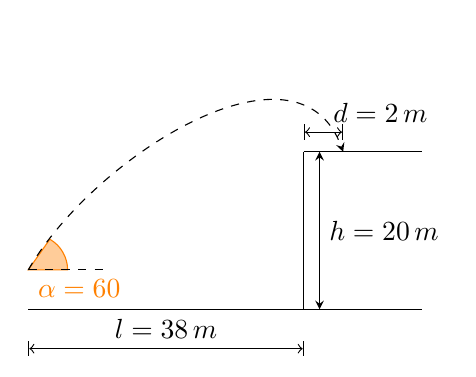
\begin{tikzpicture}
		\filldraw[orange, fill=orange!40] (0,0.5) -- (0.5,0.5) arc (0:60:0.45) -- cycle
			node[below right]{$\alpha = \ang{60}$};
		\draw[dashed, -stealth] (0,0.5) to[out=60, in=110] (4,2);
		\draw[dashed] (0,0.5) -- (1,0.5);
		
		\draw (0,0) -- (5,0);
		\draw (3.5,2) -- (3.5,0);
		\draw (3.5,2) -- (5,2);
		
		\draw[|<->|] (0,-0.5) -- ++(3.5,0)
			node[pos=0.5, above]{$l=38\,\text{m}$};
		\draw[stealth-stealth] (3.7,2) -- ++(0,-2)
			node[pos=0.5, right]{$h = 20\,\text{m}$};
		\draw[|<->|] (3.5,2.25) -- ++(0.5,0)
			node[pos=0.5, above right]{$d=2\,\text{m}$};
	\end{tikzpicture}
\end{center}

\divisor

La distanza totale che la pallina percorre è $x = l + d = 40\,\text{m}$. Quindi il tempo passato prima
dell'atterraggio è pari a 
\begin{equation*}
t = \frac{x}{v_{0_x}} \rightarrow t = \frac{x}{v_0\cos\alpha} = \frac{2x}{v_0}
\end{equation*}
Avendo poi a mente l'equazione oraria
\begin{equation*}
y = v_{0_y}t - \frac{1}{2}gt^2
\end{equation*}
possiamo sostituire le informazioni conosciute
\begin{equation*}
20 = \sin60v_0\frac{2x}{v_0} - \frac{1}{2}g\frac{2x}{v_0}^2 \rightarrow
v_0 = \frac{\sqrt{31,360}}{49.3} = \boxed{25.2\,\text{m/s}}
\end{equation*}

\paragraph{Esercizio 2}
Una pallina è lanciata verticalmente con una velocità $v_y = 10\,\text{m/s}$ da un tetto ad altezza
$h = 20\,\text{m}$. \textbf{Quanto tempo} passa prima che tocchi il terreno? \textbf{A quale velocità}
lo colipirà?

\divisor

Quanto tempo è facilmente individuabile. Prendiamo la formula oraria
\begin{equation*}
y = y_0 + v_0t+\frac{1}{2}at^2 \rightarrow y = \cancel{y_0}+\cancel{v_0t}+\frac{1}{2}at^2
\end{equation*}
Abbiamo tagliato le variabili che sono pari a $0$ nel nostro caso. Isoliamo $t$ e abbiamo
\begin{equation*}
t = \sqrt{\frac{2y}{g}}
\end{equation*}
Stiamo però attenti. Questa formula presuppone che $v_{0_y} = 0$ e nel nostro caso non è così. Però
$v_{0_y} = 0$ quando la pallina ha raggiunto l'altezza massima dopo il lancio e torna a scendere.
Infatti anche $y$ non è solo $20$ perché quando la pallina comincia a cadere ha già raggiunto una 
certa altezza. Troviamola
\begin{equation*}
h_{max} = \frac{v_{0_y}^2}{2g} \rightarrow h_{max} = \frac{100}{2\cdot9.81} = 5\,\text{m}
\end{equation*}
Possiamo ora sostituire nella formula precedente per trovare il tempo
\begin{equation*}
t = \sqrt{\frac{2y}{g}} \rightarrow t = \sqrt{\frac{2\cdot(20+5)}{9.81}} \approx\boxed{2\,\text{s}}
\end{equation*}
La velocità è ricavabile dalla formula
\begin{align*}
v^2 &= v_0^2 + 2a\Delta x \rightarrow v = \sqrt{2gh} \rightarrow\\
v &= \sqrt{2\cdot9.81\cdot25}\approx
\boxed{22.41\,\text{m/s}}
\end{align*}

\subsection*{\hyperref[sec:dinamica]{Dinamica}}\label{ex:dinamica}
\subsubsection*{\hyperref[subsec:dinamica:piano]{Funi, carrucole, piani inclinati e attrito}}
\label{ex:dinamica:piano}
\paragraph{Esercizio 1}
Un corpo di massa $2\,\text{kg}$ scivola lungo un piano inclinato liscio (senza attrito). Determina \\
l'\textbf{accelerazione} con la quale si muove e il \textbf{tempo} che impiega a percorrere tutto il
piano, sapendo che la lunghezza del piano è $1\,\text{m}$ e la sua altezza è $0.5\,\text{m}$.
\divisor

L'accelerazione è veramente semplice trovarla in quanto basta ricordarsi una formula:
\begin{equation*}
a = g\sin\alpha \rightarrow a = 9.81\cdot\sin\ang{30} = 9.81 \cdot 0.5 = \boxed{4.905\,\text{m/s}^2}
\end{equation*}
Come sapevamo l'angolo? Essendo il piano inclinato l'ipotenusa, la trigonometria dice che perché
l'altezza sia di $0.5$ l'angolo deve essere di $\ang{30}$.\\[\baselineskip]
E ora, avendo l'accelerazione è un semplice esercizio di cinematica. Per prima cosa si trova la
velocità finale usando una delle formule più utili di sempre
\begin{align*}
v^2= v_0^2+2a\cdot\Delta x \rightarrow v^2 = 0^2 + 2\cdot4.905\cdot1 = 9.81 \rightarrow\\
v = \sqrt{v^2} = \sqrt{9.81} \approx \underline{3.31\,\text{m/s}}
\end{align*}
e ora si trova il tempo
\begin{equation*}
v = v_0 + at \rightarrow t = \frac{v-v_0}{a} \rightarrow t = \frac{3.13}{4.905} \approx 
\boxed{0.64\,\text{s}}
\end{equation*}

\paragraph{Esercizio 2}
Un blocco A di massa $M = 0.6\,\text{kg}$ si muove senza attrito su un piano inclinato di $\ang{30}$. 
Mediante una fune priva di massa, il blocco A è connesso ad un blocco B di $22.0\,\text{kg}$ come 
mostrato in figura. La carrucola ha massa trascurabile e si muove senza attrito. Determina 
l'\textbf{accelerazione} di ciascun blocco e la \textbf{tensione} della corda.

\begin{center}
	\begin{tikzpicture}
	\coordinate (A) at (0,0);
	\coordinate (B) at (5,0);
	\coordinate (C) at (0,2);
	\coordinate (D) at ($(C) + (-0.2, 0.2)$); % Circle center
	\coordinate (M1) at ($(D) + (-0.2, -0.5)$);
	\coordinate (M2) at ($(D) + (1, -0.25)$);
	
	\draw[very thin] (A) -- (B) -- (C) -- cycle; % Triangle
	\filldraw[orange, fill=orange!30] (B) -- ($(B) + (-1, 0)$) arc(180:158:1) -- cycle
	node[pos=0, below left]{$\alpha$}; % Arc
	\filldraw[fill=teal!20, very thin] (D) circle (0.2)
	node[teal]{$m$}; % Circle
	\draw[very thin] (D) -- (C); % Line from C to circle
	\draw[very thin] ($(D) + (-0.2, 0)$) -- (M1);
	\draw[red] ($(M1) + (-0.2, 0)$) -- ($(M1) + (-0.2, -0.3)$) -- ($(M1) + (0.2, -0.3)$) --
	($(M1) + (0.2, 0)$) -- cycle
	node[pos=0.5, below]{$B$}; % Box 1
	\draw[very thin] ($(D) + (0.15, 0.15)$) -- (M2);
	\draw[blue] ($(M2) + (0.1, 0.2)$) -- ($(M2) + (0.5, 0.01)$) -- ($(M2) + (0.35, -0.4)$) --
	($(M2) + (-0.1, -0.2)$) -- cycle
	node[pos=0, right]{$A$};
	\end{tikzpicture}
\end{center}
\divisor

Si trova l'accelerazione molto rapidamente mediante l'uso di una singola formula:
\begin{align*}
a = \frac{m_Bg - m_A\sin\alpha}{m_A+m_B} \rightarrow a =
\frac{22\cdot9.81-8\cdot9.81\cdot\sin\ang{30}}{22+8}\rightarrow\\
a = \frac{215.82 - 39.24}{31} \rightarrow \frac{176.58}{31} \approx \boxed{5.69\,\text{m/s}^2}
\end{align*}
Per la tensione la questione è un po' più particolare. La tensione rappresenta la risultante
tra la forza che tira da ciascuna parte. Quindi, per prima cosa troviamole
\begin{equation*}
F_A = m_A\sin\alpha \rightarrow F_A = 8\cdot9.81\sin\ang{30} = \underline{39.24\,\text{N}}
\end{equation*}
\begin{equation*}
F_B = m_Bg \rightarrow F_B = 22\cdot9.81 = \underline{215.82\,N}
\end{equation*}
Ora per trovare la tensione vediamo che il blocco che "tira" è il blocco B. Quindi
\begin{equation*}
T = \frac{F_B-F_A}{2} \rightarrow T = \frac{215.82-39.24}{2} = \boxed{88.29\,\text{N}}
\end{equation*}
Da notare che si divide per due in quanto la tensione che troviamo è da entrambe le parti, a noi
interessa solo una.

\paragraph{Esercizio 3}
Considera il sistema di blocchi $m_1 = 80.0\,\text{kg}$, $m_2 = 90\,\text{kg}$ tirati da una massa 
$m_3 = 60\,\text{kg}$. Se il coefficiente di attrito dinamico tra le superfici dei blocchi e il 
binario orizzontale vale $\mu_d = 0.3$, determina \textbf{l'accelerazione} del sistema e le 
\textbf{tensioni} dei fili.

\begin{center}
	\begin{tikzpicture}
		\coordinate (m1) at (0,0);
		\coordinate (m2) at (2,0);
		\coordinate (m3) at (4.8,-2);
		
		\draw (-2,-0.5) -- (4.1,-0.5) -- (4.1,-4);
		\draw (4.1,-0.5) -- ++(0.3,0.2);
		\draw (4.6,-0.2) circle (0.2);
		
		\draw ($(m1) + (-0.5,0.5)$) -- ++(1,0) -- ++(0,-1) -- ++(-1,0) -- cycle;
		\draw ($(m2) + (-0.5,0.5)$) -- ++(1,0) -- ++(0,-1) -- ++(-1,0) -- cycle;
		\draw ($(m3) + (-0.5,0.5)$) -- ++(1,0) -- ++(0,-1) -- ++(-1,0) -- cycle;
		\draw ($(m1) + (0.5,0)$) -- ($(m2) + (-0.5,0)$);
		\draw ($(m2) + (0.5,0)$) -- ++(2.1,0);
		\draw (4.8,-0.2) -- ($(m3) + (0,0.5)$);
		
		\node (m) at (m1){$m_1$};
		\node (m) at (m2){$m_2$};
		\node (m) at (m3){$m_3$};
	\end{tikzpicture}
\end{center}
\divisor

Per risolvere questo tipo di esercizi, bisogna essere metodici. Per prima cosa troviamo la forza
peso di $m_3$ che è anche l'unica forza che agisce direttamente.
\begin{equation*}
P = m\cdot g \rightarrow P = 60\cdot9.81 = \underline{588.6\,\text{N}}
\end{equation*}
Ora noi utilizzeremo la definizione di forza per calcolare l'accelerazione. Quindi dobbiamo vedere
la forza che agisce direttamente sul sitema. Per ora abbiamo calcolato $P$, però in contrasto
ci sono anche le forze di attrito. Calcoliamole.
\begin{equation*}
F_{a_1} = P_1\cdot\mu_d \rightarrow F_{a_1} = 80\cdot9.81\cdot0.3 = \underline{235.44\,\text{N}}
\end{equation*}
\begin{equation*}
F_{a_2} = P_2\cdot\mu_d \rightarrow F_{a_2} = 90\cdot9.81\cdot0.3 = \underline{264.87\,N}
\end{equation*}
E ora possiamo trovarci la forza che agisce sul sistema. Dato che le forze di attrito contrastano
la forza peso, si tolgono da quest'ultima.
\begin{align*}
F = \sum F \rightarrow F = P - F_{a_1} - F_{a_2} \rightarrow\\
F = 588.6 - 235.44 - 264.87 = \underline{88.29\,\text{N}}
\end{align*}
E infine sfruttando la definizione di forza, possiamo ricavare l'accelerazione.
\begin{equation*}
F = ma \rightarrow a = \frac{F}{m} \rightarrow a = \frac{88.29}{80+90+60} 
\approx\boxed{0.38\,\text{m/s}^2}
\end{equation*}
Per le tensioni possiamo immediatamente trovare $T_1$ in quanto è l'unica che agisce su $m_1$ che è
isolato.
\begin{equation*}
T_1 = a\cdot m_1 \rightarrow T_1 = 0.38\cdot80 = \boxed{30.4\,\text{N}}
\end{equation*}
E quesat è la prima, la seconda invece richiede un attimo di attenzione. Su $m_2$ agiscono sia $T_1$ 
che $T_2$. Dato che sappiamo che il sistema non è in equilibrio (è presente un'accelerazione),
sappiamo anche che le $T_2-T_1 = m_2\cdot a$ in quanto sul corpo $m_2$ è presente l'accelerazione e
agiscono le due tensioni.
\begin{align*}
T_2-T_1 = m_2\cdot a \rightarrow T_2 = T_1 + m_2\cdot a \rightarrow\\
T_2 = 30.4 + 90\cdot0.38 = \boxed{64.6\,\text{N}}
\end{align*}

\paragraph{Esercizio 4}
Una scala uniforme è appoggiata al muro, formando un angolo $\theta$ con il pavimento. Il coefficiente
di attrito tra la scala e il pavimento è $\mu$. \textbf{Trova in funzione di $\mu$ l'angolo minimo
$\theta_m$ in cui la scala non scivola.}
\divisor

Disegnando la situazione con anche le forze in gioco risulta
\begin{center}
	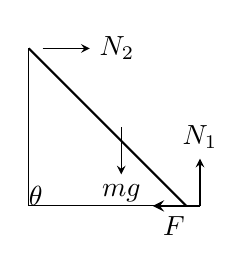
\begin{tikzpicture}[scale=2]
		\coordinate (N1) at (0,1);
		\coordinate (N2) at (1,0);
		\coordinate (O) at (0,0);
		\coordinate (M) at (0.5,0.5);
		
		\draw (O) -- (N1);
		\draw (O) -- (N2);
		\draw[thick] (N1) -- (N2);
		
		\markangle{N2}{O}{N1}{0.3}{1.3}{$\theta$}
		\draw[-stealth] (N1) -- +(0.3,0)
			node[pos=1, right]{$N_2$};
		\draw[-stealth] (N2) -- +(0,0.3)
			node[pos=1, above]{$N_1$};
		\draw[-stealth] (M) -- ++(0,-0.3)
			node[pos=1, below]{$mg$};
		\draw[thick,-stealth] (N2) -- +(-0.3,0)
			node[pos=1, below right]{$F$};
	\end{tikzpicture}
\end{center}
Quindi siano $N_1$ e $N_2$ le forze di reazione contro la scala e $F$ la forza di attrito che tiene su
la scala. Diciamo che la scala è lunga $L$ e ha massa $m$. Allora la condizione di equlibrio è data
da
\begin{equation*}
\sum F_x = 0 \qquad \sum F_y = 0
\end{equation*}
quindi
\begin{equation*}
\begin{cases}
N_2-F=0\\
N_1-mg=0
\end{cases}
\end{equation*}
Scegliamo ora un punto di riferimento: il punto di contatto tra la scala e il pavimento. Decidiamo
poi che se una forza si allontana dal muro è negativa. Quindi le forze che agiuscono in quel punto
devono essere zero (per la condizione di equilibrio). Quindi
\begin{equation*}
-LN_2\sin\theta + \overbrace{\frac{L}{2}}^{\mathclap{\text{Questo perché la massa si trova nel 
baricentro (o centro di massa)}}}mg\cos\theta = 0
\end{equation*}
che semplificato diventa
\begin{equation*}
N_2\tan\theta = \frac{1}{2}mg
\end{equation*}
Utilizzando la prima equazione del sistema, possiamo quindi dire che
\begin{equation*}
\frac{1}{2}mg\tan\theta=F
\end{equation*}
L'equilibrio è possibile fintanto che $F\leq N_1\mu$. Usando la seconda equazione viene che
\begin{equation*}
N_1\mu = mg\mu
\end{equation*}
quindi l'equilibrio necessita che $\tan\theta\leq\frac{1}{2}\mu$ e quindi
\begin{equation*}
\boxed{\theta_m = \arctan\frac{1}{2}\mu}
\end{equation*}

\subsubsection*{\hyperref[subsec:dinamica:potenziale]{Lavoro, Energia e Potenza}}\label{ex:potenziale}
\paragraph{Esercizio 1}
Un ragazzo su uno skateboard parte nel punto A rappresentato in figura, e sale fino ad un'altezza
di $2.64\,m$ al di sopra dell'estremità della rampa nel punto B. Qual era il modulo della
\textbf{velocità} iniziale del ragazzo nel punto A?

\begin{center}
	\begin{tikzpicture}
		\draw (0,0) to[out=-90,in=-90] (4,0);
		\draw[dashed] (0,0) -- (4,0)
			node[pos=0, above]{A};
		\draw[|<->|, densely dotted] (4,0) -- (4,1)
			node[pos=0.5, right]{$2.64\,m$}
			node[pos=1, left]{B};
	\end{tikzpicture}
\end{center}
\divisor

Siamo in un caso di sistema conservativo e quindi possiamo sfruttare la formula $U_1+E_{c_1} = 
U_2 + E_{c_2}$. Sfruttando questa caratteristica possiamo semplicemente risolvere.
\begin{equation*}
U_1+E_{c_1} = U_2 + E_{c_2} \rightarrow mgh_1 + \frac{1}{2}mv_1^2 = mgh_2 + \frac{1}{2}mv_2^2
\end{equation*}
Ora però, prima di passare ai calcoli, possiamo subito semplificare la formula in quanto sappiamo
che nel secondo momento il ragazzo si ferma quando raggiunge i $2.64\,m$. Quindi semplifichiamola.
\begin{align*}
mgh_1 + \frac{1}{2}mv_1^2 = mgh_2 + \frac{1}{2}mv_2^2 \rightarrow \\
mgh_1 + \frac{1}{2}mv_1^2 = mgh_2 + \cancel{\frac{1}{2}mv_2^2} \rightarrow\\
\cancel{m}gh_1 + \frac{1}{2}\cancel{m}v_1^2 = \cancel{m}gh_2 \rightarrow
gh_1 + \frac{1}{2}v_1^2 = gh_2
\end{align*}
Abbiamo anche cancellato la $m$ in quanto è costante a tutti gli elementi.\\
Ora possiamo sostituire a $h_2$ il suo valore effettivo, ovvero $h_1+2.64$. Questo perché non 
sappiamo a che altezza parte ma sappiamo che la supera di $2.64\,m$.
\begin{align*}
gh_1 + \frac{1}{2}v_1^2 = gh_2 \rightarrow gh_1 + \frac{1}{2}v_1^2 = g\left(h_1+.64\right)\\
gh_1 + \frac{1}{2}v_1^2 = gh_1 + g\cdot2.64
\end{align*}
E ora non ci resta che isolare $v$.
\begin{align*}
gh_1 + \frac{1}{2}v_1^2 = gh_1 + g\cdot2.64 \rightarrow
\frac{1}{2}v_1^2 = \cancel{gh_1} + g\cdot2.64 -\cancel{gh_1} \rightarrow\\
v_1^2 = 9.81\cdot2.64\cdot2 \rightarrow\\
v_1 = \sqrt{9.81\cdot2.64\cdot2} = \sqrt{51.8}
\approx\boxed{7.2\,\text{m/s}}
\end{align*}

\paragraph{Esercizio 2}
Un pendolo semplice ha la lunghezza di $.75\,\text{m}$ e una pallina con una massa d 
$0.15\,\text{kg}$. La pallina viene lasciata andare quando il filo forma un angolo di $\ang{25}$ 
rispetto alla verticale.
\begin{itemize}[label={$\bullet$}]
	\item \textbf{Dimostra} che l'altezza da cui la pallina del pendolo viene lasciata andare è 
	$h=l\cdot(1-\cos\ang{25})$
	\item Qual è l'\textbf{energia cinetica} del pendolo quando, durante l'oscillazione, il filo 
	forma un angolo di $\ang{9.0}$?
	\item Qual è la \textbf{velocità} del pendolo nel punto più basso della sua oscillazione?
\end{itemize}

\begin{center}
	\begin{tikzpicture}
		\coordinate (Top) at (0,3);
		\coordinate (Ball) at (1,.1);
		\coordinate (H) at (0,-0.1);
		
		\draw (Top) -- (Ball);
		\draw[dashed] (Top) -- ++(0,-4);
		\draw[dashed] (Ball) -- ++(-1,0);
		\draw[dashed] (Ball) to[out=190, in=0] (H);
		\draw (Top) -- ++(0,-0.8) arc (-90:-75:1)
			node[pos=0.5, below]{$\ang{25}$};
		\draw[|<->|] ($(Top) + (0.4, 0.)$) -- ($(Ball) + (0.4,0.)$)
			node[pos=0.5, right]{$l = 0.75\,m$};
		\draw[|<->|] ($(H) + (-0.2,0.)$) -- ($(Ball) + (-1.2,0.)$)
			node[pos=0.5, left]{$h$};
		
		\filldraw[gray] (Ball) circle (0.2);
	\end{tikzpicture}
\end{center}
\divisor

Dimostrare il primo punto è estremamente semplice e richiede solo nozioni di trigonometria. Il
successivo disegno aiuterà a chiarire:
\begin{center}
	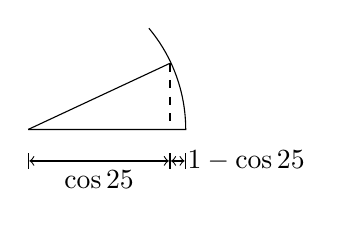
\begin{tikzpicture}[scale=2]
		\draw (0,0) -- (1,0);
		\draw (0,0) -- (0.9,0.42);
		\draw[dashed] (0.9,0.42) -- ++(0,-0.42);
		\draw (0,0) -- (1,0) arc (0:40:1);
		\draw[|<->|] (0,-0.2) -- ++(0.9,0)
			node[pos=0.5, below]{$\cos\ang{25}$};
		\draw[|<->|] (0.9,-0.2) -- ++(0.1,0)
			node[pos=0.5, right]{$1-\cos\ang{25}$};
	\end{tikzpicture}
\end{center}
Come si può vedere, la lunghezza $1-\cos\ang{25}$ è il nostro $h$. Quindi perché moltiplicarla per 
$l$? Perché la lunghezza della corda non è quella della circonferenza goniometrica ($0.75 \neq 1$).\\
Avendo quindi chiarito il primo punto, possiamo concentrarci sul secondo.\\[\baselineskip]

Per prima cosa, ricordando la formula per l'energia cinetica ($E_c = \dfrac{1}{2}mv^2$) notiamo che ci
manca solo la velocità. Come trovarla? Utilizando la solita formula $U_1+E_{c_1} = U_2 + E_{c_2}$.
\begin{equation*}
U_1+E_{c_1} = U_2 + E_{c_2} \rightarrow mgh_1 + \frac{1}{2}mv_1^2 = mgh_2 + \frac{1}{2}mv_2^2
\end{equation*}
Prima di proseguire i calcoli, possiamo subito eliminare due dei quattro elementi.
\begin{align*}
mgh_1 + \frac{1}{2}mv_1^2 &= mgh_2 + \frac{1}{2}mv_2^2 \rightarrow\\
mgh_1 + \cancel{\frac{1}{2}mv_1^2} &= \cancel{mgh_2} + \frac{1}{2}mv_2^2 \rightarrow\\
\cancel{m}gh_1 &= \frac{1}{2}\cancel{m}v_2^2
\end{align*}
Possiamo ora trovarci la velocità. Non serve neanche facciamo la radice quadrata in quanto dopo 
comunque lo ri-eleveremmo al quadrato.
\begin{align*}
gh_1 &= \frac{1}{2}v_2^2 \rightarrow \\
v_2^2 &= 2\cdot9.81\cdot(1-\cos\ang{25})\cdot0.75 = 
\underline{13.3416\,\text{m/s}}
\end{align*}
E ora troviamo l'energia cinetica
\begin{equation*}
E_c = \frac{1}{2}mv^2 \rightarrow \frac{1}{2}\cdot0.15\cdot13.3416 = \boxed{1\,\text{J}}
\end{equation*}
Ora manca solo l'ultimo punto. La teoria è molto simile alla prima parte, in definitiva cambia solo 
l'altezza.
\begin{align*}
mgh_1 + \frac{1}{2}mv_1^2 &= mgh_2 + \frac{1}{2}mv_2^2 \rightarrow\\
mgh_1 + \cancel{\frac{1}{2}mv_1^2} &= \cancel{mgh_2} + \frac{1}{2}mv_2^2 \rightarrow\\
\cancel{m}gh_1 &= \frac{1}{2}\cancel{m}v_2^2 \rightarrow
v = \sqrt{2\cdot9.81\cdot0.75} \approx \boxed{3.83\text{m/s}}
\end{align*}

\paragraph{Esercizio 3}
Una gru solleva un peso di massa $m = 500\,\text{kg}$ verticalmente a velocità costante 
$v = 2\,\text{m/s}$. Trova la \textbf{potenza spesa dal motore della gru}. Qual è il \textbf{lavoro}
fatto dalla gru se solleva il peso di $h = 20\,\text{m}$?\\
Una seconda gru è capace di sollevare la stessa massa al doppio della velocità. Trova la potenza
e il lavoro fatti dalla seconda gru alzando il peso della stessa altezza.

\divisor

Il lavoro è definito come $L = F\cdot S\cdot \cos\alpha$ e quindi sostituendo ciò che abbiamo
\begin{equation*}
L = F\cdot S\cdot \cos\alpha \rightarrow L = 500\cdot9.81\cdot20\cdot\cos90 = 
\boxed{98100\,\text{N}\cdot\text{m}}
\end{equation*}
Per trovare la potenza abbiamo bisogno anche del tempo. Troviamolo
\begin{equation*}
x = x_0 +vt \rightarrow 20 = 0+2t \rightarrow t = 10\,\text{s}
\end{equation*}
La potenza può essere trovata facilmente usando l'altra formula per il lavoro
\begin{equation*}
P = \frac{L}{t} \rightarrow P = \frac{98100}{10} = \boxed{9800\,\text{W}}
\end{equation*}
Per l'ultimo punto, dato che abbiamo una forza costante che agisce, possiamo usare la seguente formula
\begin{equation*}
P = Fv \rightarrow P = mav\rightarrow 500\cdot9.81\cdot4 = \boxed{19620\,\text{W}}
\end{equation*}
La formula si ricava da $\frac{F\cdot S}{t}\rightarrow Fv$.\\
Il lavoro lo si trova esattamente come prima
\begin{equation*}
L = F\cdot S\cdot \cos\alpha \rightarrow L = 500\cdot9.81\cdot20\cdot\cos90 = 
\boxed{98100\,\text{N}\cdot\text{m}}
\end{equation*}
Notiamo allora che il lavoro rimane costante mentre la potenza raddoppia.

\subsubsection*{\hyperref[subsec:dinamica:impulso]{Impulso}}\label{ex:impulso}
\paragraph{Esercizio 1}
Una barca e i suoi occupanti di massa $M = 200\,\text{kg}$ contiene $10$ sacchi di carbone ciascuno di
$5\,\text{kg}$. La barca è stazionaria nella sua posizione. Gli occupanti cercano di raggiungere la
riva lanciando fuori i sacchi di carbone ad una velocità orizzontale relativa $v_r$. Assumendo 
l'attrito nullo, \textbf{qual è la velocità dopo il primo sacco}? \textbf{E dopo il secondo?} Scrivi
i risultati in termini di $v_r$.
\divisor

Innanzitutto sappiamo che il sistema è conservativo in quanto non ci sono forze esterne. Detto questo,
sappiamo anche che quindi $q_1 = q_2$. Prima di cominciare, sappiamo che il sistema ha massa 
$200+5\cdot10$\\
Nel primo caso vediamo che la barca è ferma quindi sappiamo già che $q_1 = 0$. Quindi possiamo 
scrivere
\begin{align*}
&0 = 245v - 5v_r\rightarrow v = \frac{5v_r}{245} = \boxed{\frac{1}{43}v_r}
\end{align*}
$245$ perché nella situazione finale è che la barca ha perso una sacca ed essa sta volando. Sappiamo 
quindi la velocità nel primo caso.\\
Nel secondo caso, la barca ha già una sua velocità quindi scriviamo
\begin{align*}
&\frac{1}{43}v_r = 240v + 5\left(-v_r + \frac{1}{43}v_r\right)
\intertext{Isoliamo $v$ e otteniamo}
&\boxed{v \approx 4\cdot10^{-2}\,\text{m/s}}
\end{align*}
Abbiamo risolto il problema ma perché abbiamo scritto $-v_r + \dfrac{1}{43}v_r$? Nella seconda 
situazione la barca ha già una velocità propria che è opposta a quella che ottiene il sacco lanciato.
La situazione è simile a quella di un treno in corsa da cui si spara un proiettile in verso opposto.
Ci stiamo spostando ad una velocità pari a $\dfrac{1}{43}v_r$ e la sacca ha velocità in verso opposto
pari a $v_r$.

\subsubsection*{\hyperref[subsec:dinamica:urti]{Urti}}\label{ex:urti}
\paragraph{Esercizio 1}
Una mitragliatrice di massa $30\,\text{kg}$ (comprendente quella dei proiettili) è installata a bordo 
di un carrello di massa $100\,\text{kg}$ e spara verso sinistra una sventagliata di $10$ proiettili 
ciascuno di massa $30\,g$ con la velocità di $60\,\text{m/s}$. Quale \textbf{velocità} verso destra 
acquisterà il carrello?
\divisor

Qui siamo in un caso in di urto elastico, quindi vige il principio di conservazione del moto. Di
conseguenza la soluzione di quest'esercizio è estremamente semplice.
\begin{equation*}
m_1v_1 = m_2v_2 \rightarrow 60\cdot0.30 = 129.7\cdot v_2
\end{equation*}
Perché $129.7$? Perché sappiamo che la mitragliatrice e il carrello pesano insieme $100 + 30 = 
130\,Kg$ ma sono stati sparati $10$ colpi da $0.03\,Kg$  l'uno, quindi il peso finale sarà
$130 - 10\cdot0.03 = 129.7\,Kg$.\\
Ora non resta che risolvere semplicemente.
\begin{equation*}
v_2 = \frac{60\cdot0.30}{129.7} \approx\boxed{0.139\,\text{m/s}}
\end{equation*}

\paragraph{Esercizio 2}
Una pallottola di massa $m = 10\,g$ colpisce alla velocità $v_p = 280\,m/s$ un pendolo balistico di
massa $M = 2.0\,Kg$, restando incorporata nel pendolo. Calcola l'\textbf{altezza} $h$ di cui s'innalza
il pendolo.
\divisor

Questo esercizio è estremamente semplice in quanto siamo in una situazione di un proiettile contro
un corpo e abbiamo tutti i dati necessari.
\begin{align*}
v_p = \frac{M+m}{m}\sqrt{2gh} \rightarrow h &= \frac{v_p^2m^2}{2g\left(M+m\right)^2} \rightarrow\\
h = \frac{280^2\cdot0.01^2}{2\cdot9.81\cdot(2+0.01)^2} \rightarrow h &= \frac{7.84}{86.5242} = 
\boxed{0.09\,\text{m}}
\end{align*}

\subsubsection*{\hyperref[subsec:dinamica:cm]{Centro di Massa}}\label{ex:cm}
\paragraph{Esercizio 1}
Una racchetta da tennis può essere schematizzata in un cerchio di raggio $r$ e massa $m_1 $ a cui è 
attaccato un bastone uniforme di lunghezza $l$ e massa $m_1$. Ponendo $r = l/2$ e $m_1=m_2$, trova il
\textbf{centro di massa} della racchetta. Viene poi aggiunta una massa $m_3 = m_2/2$ nel punto più
lontano dal bastone. Trova il \textbf{nuovo centro di massa}.

\begin{center}
	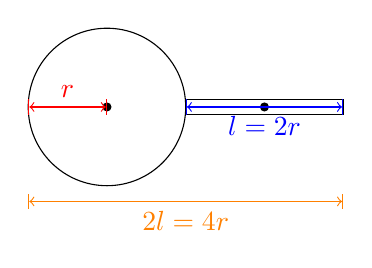
\begin{tikzpicture}
		\draw (0,0) circle (1);
		\filldraw[white, draw=black] (1,0.1) -- ++(2,0) -- ++(0,-0.2) -- ++(-2,0) -- cycle;
		\filldraw (0,0) circle (0.05);
		\filldraw (2,0) circle (0.05);
		\draw[|<->|, red] (-1,0) -- (0,0)
			node[pos=0.5, above]{$r$};
		\draw[|<->|, blue] (1,0) -- (3,0)
			node[pos=0.5, below]{$l = 2r$};
		\draw[|<->|, orange] (-1,-1.2) -- (3,-1.2)
			node[pos=0.5, below]{$2l = 4r$};
	\end{tikzpicture}
\end{center}

\divisor

Sappiamo che in un corpo uniforme il centro di massa si trova nel baricentro. Nel caso del cerchio è
nel centro stesso e nel caso del rettangolo è a a metà della sua lunghezza. Dato che abbiamo due 
possibilità, scegliamo di scrivere tutto in funzione di $r$. È generalmente meglio scegliere la \\
variabile più "piccola" perché dona più flessibilità. Decidiamo anche di porre l'origine al manico 
della racchetta.\\
A questo punto procediamo con i calcoli. Dal disegno vediamo già tutte le distanze
\begin{equation*}
x = \frac{\sum xm}{\sum m} \rightarrow x = \frac{m\cdot r + m\cdot 3r}{2m} \rightarrow
x = \frac{4rm}{2m} = \boxed{2r}
\end{equation*}
Il centro di massa si trova quindi all'attaccatura del manico.\\
Aggiunta la nuova massa, aggiorniamo i calcoli
\begin{align*}
x &= \frac{\sum xm}{\sum m} \rightarrow 
x=\frac{\frac{m}{2}4r + m\cdot r + m\cdot 3r}{2m+\frac{m}{2}}\rightarrow\\
x &= \frac{7mr}{\frac{5}{2}m} \rightarrow x = \boxed{\frac{14}{5}r}
\end{align*}

\subsubsection*{\hyperref[subsec:dinamica:inerzia]{Momento Angolare ed Inerzia}}\label{ex:inerzia}
\paragraph{Esercizio 1}
Una penna di lunghezza $12\,\text{cm}$ viene appoggiata in posizione verticale su un piano con 
attrito. Essa inizialmente ferma, cade ruotando attorno al punto di contatto con il piano. Calcola
\textbf{la velocità lineare} della testa della penna e l'\textbf{accelerazione angolare} nell'istante 
dell'impatto con il piano.
\divisor

Essendo un problema di dinamica in cui il sistema è conservativo, possiamo scrivere subito
\begin{equation*}
U_1 + E_{c_1} = U_2 + E_{c_2}
\end{equation*}
In questo modo possiamo anche subito eliminare due elementi. Sappiamo che parte da ferma e arriva ad
essere ferma. Questo significa che all'inizio c'è solo energia potenziale, alla fine solo cinetica.
\begin{equation*}
U_1 + E_{c_1} = U_2 + E_{c_2} \rightarrow U_1 + \cancel{E_{c_1}} = \cancel{U_2} + E_{c_2}
\end{equation*}
Quindi ora abbiamo un'equazione in cui possiamo cominciare a sostituire
\begin{equation*}
U_1 = E_{c_2} \rightarrow mg\frac{l}{2} = \frac{1}{2}I\omega^2
\end{equation*}
Come mai $\frac{l}{2}$ e non $l$? Questo perché l'energia si concentra nel centro di massa che si 
trova a metà distanza tra la punta e la testa della penna. Ora possiamo sostituire a $I$ l'inerzia
di una barra che è equivalente a $\dfrac{1}{12}ml^2 + m\dfrac{l^2}{4}$
\begin{gather*}
\frac{1}{2}mgl = \frac{1}{2}\left(\frac{1}{12}ml^2 + m\frac{l^2}{4}\right)\omega^2 \rightarrow\\
\cancel{\frac{1}{2}}\cancel{m}gl = \cancel{\frac{1}{2}}\left(\frac{1}{3}\cancel{m}l^2\right)\omega^2 
\rightarrow\\
g\cancel{l} = \frac{1}{3}l^{\cancel{2}}\omega^2 \rightarrow \omega = \sqrt{\frac{3g}{l}} \rightarrow\\
\omega = \sqrt{\frac{3\cdot9.81}{0.12}} \approx \underline{15.6\,\text{rad/s}}
\end{gather*}
E ora non resta che trovare la velocità tangenziale avendo quella angolare
\begin{equation*}
v = \omega r \rightarrow v = 15.6\cdot0.12 = \boxed{1.8\,\text{m/s}}
\end{equation*}
E ora è da trovare solo l'accelerazione angolare. Anche qui sfruttiamo la conservitività del sistema.
\begin{equation*}
\frac{1}{2}\cancel{m}g\cancel{l} = \frac{1}{3}\cancel{m}l^{\cancel{2}}\alpha \rightarrow
\alpha = \frac{3g}{2l} \rightarrow \alpha = \frac{3\cdot9.81}{2\cdot0.12} = 
\boxed{122.6\,\text{rad/s}^2}
\end{equation*}

\paragraph{Esercizio 2}
Una ruota è costituita da un anello di spessore trascurabile di massa $M=20\,\text{kg}$, sostenuto da 
raggi di massa trascurabile e di lunghezza $R = 0.5\,\text{m}$. Essa sta ruotando attorno al proprio
asse alla frequenza di $5\,\text{Hz}$. Alla sua periferia viene accostata una piastra con la quale 
essa sviluppa una forza di $50\,\text{N}$ tangente alla ruota. Determinare \textbf{quanti giri} deve 
compiere la ruota prima di fermarsi.
\divisor

Per prima cosa identifichiamo che abbiamo un corpo che ruota e una forza che generano un momento. 
Quindi troviamoci quanto vale la decelerazione causata da questa forza tangenziale
\begin{gather*}
M = I\alpha \rightarrow -F_a\cancel{r} = mr^{\cancel{2}}\alpha \rightarrow
\alpha = \frac{-F_a}{mr} \rightarrow \\\alpha -\frac{50}{20\cdot0.5} = \underline{-5\,\text{rad/s}^2}
\end{gather*}
Ora possiamo facilmente trovarci la velocità angolare così poi da poter usare la legge oraria
\begin{equation*}
\omega = \frac{2\pi}{T} \rightarrow \omega = \frac{2\pi}{\frac{1}{f}} \rightarrow \omega = 2\pi f
\rightarrow \omega = \underline{10\pi}
\end{equation*}
Per comodità per ora non approssimiamo. Ora se vogliamo usare la seguente legge oraria
\begin{equation*}
\theta = \theta_0+\omega_0t+\frac{1}{2}\alpha t^2
\end{equation*}
dobbiamo trovare il tempo $t$.
\begin{equation*}
\omega = \omega_0 + \alpha t \rightarrow t = \frac{\omega-\omega_0}{\alpha} \rightarrow
t = \frac{0 - 10\pi}{-5} = \underline{2\pi\,\text{s}}
\end{equation*}
E ora abbiamo tutto ciò che ci serve.
\begin{gather*}
\theta = \theta_0+\omega_0t+\frac{1}{2}\alpha t^2 \rightarrow\\
\theta = \cancel{\theta_0}+\omega_0t+\frac{1}{2}\alpha t^2
\end{gather*}
Perché abbiamo cancellato quell'elemento? Beh, noi vogliamo sapere quanti giri, quindi partiamo da
una posizione $theta_0 = 0$. Continuiamo la risoluzione
\begin{gather*}
\theta = \omega_0t+\frac{1}{2}\alpha t^2 \rightarrow
\theta = 10\pi\cdot2\pi + \frac{1}{2}\cdot-5\cdot4\pi^2\\
\theta = 20\pi^2 - 5\cdot2\pi^2 \rightarrow \theta = 20\pi^2-10\pi^2 = 10\pi^2 \rightarrow \\
\theta = 10\cdot3.14^2 = \boxed{98.69\,\text{rad}}
\end{gather*}
Dato che ci vengono chiesti i giri, semplicemente dividiamo per $2\pi$
\begin{equation*}
\text{giri } = \frac{98.69}{2\pi} = \boxed{15.7\,\text{giri}}
\end{equation*}
	
\subsection*{\hyperref[sec:gravitazione]{Gravitazione}}\label{ex:gravitazione}
\paragraph{Esercizio 1}
La figura mostra tre corpi allineati che sono molto lontani da qualsiasi altro corpo. Le loro masse 
sono:
\begin{itemize}[label={$\bullet$}]
	\item $m_A = 363\,\text{kg}$
	\item $m_B = 517\,\text{kg}$
	\item $m_C = 154\,\text{kg}$
\end{itemize}
Determina \textbf{modulo}, \textbf{direzione} e \textbf{verso} della forza gravitazionale totale 
che agisce su ciascuno di essi.
\begin{center}
	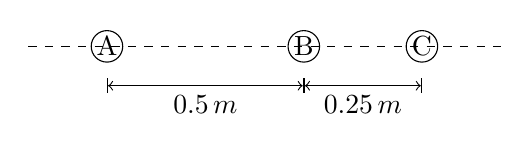
\begin{tikzpicture}
		\draw[dashed] (0,0) -- (6,0);
		\draw (1,0) circle (0.2) node{A};
		\draw (3.5,0) circle (0.2) node{B};
		\draw (5,0) circle (0.2) node{C};
		\draw[|<->|] (1,-0.5) -- (3.5,-0.5)
			node[pos=0.5, below]{$0.5\,m$};
		\draw[|<->|] (3.5,-0.5) -- (5,-0.5)
			node[pos=0.5, below]{$0.25\,m$};
	\end{tikzpicture}
\end{center}
\divisor

Ricordando la formula della forza gravitazionale, possiamo semplicemente sommare i vettori forza fra
di loro.
\begin{align*}
F &= G\frac{m_1m_2}{r^2} \rightarrow \\
&\begin{cases*}
F_{AB}  = 6.67\cdot10^{-11}\cdot\dfrac{363\cdot517}{0.5^2}\\
F_{AC}  = 6.67\cdot10^{-11}\cdot\dfrac{363\cdot154}{0.75^2}
\end{cases*} \rightarrow\\
&\begin{cases*}
F_{AB}  = 5\cdot10^{-5}\\
F_{AC}  = 6.62\cdot10^{-6}
\end{cases*} \rightarrow\\
F &= 5\cdot10^{-5}+6.62\cdot10^{-6} = \\&
\boxed{5.62\cdot10^{-5}\,\text{N}}
\end{align*}
Questo era per il corpo A. Il procedimento è identico per il corpo C, cambia leggermente per il 
corpo B.
\begin{align*}
F &= G\frac{m_1m_2}{r^2} \rightarrow\\
&\begin{cases*}
F_{BA} = 6.67\cdot10^{-11}\cdot\dfrac{517\cdot363}{0.5^2}\\
F_{BC} = 6.67\cdot10^{-11}\cdot\dfrac{517\cdot154}{0.25^2}
\end{cases*} \rightarrow\\
&\begin{cases*}
F_{BA}  = 5\cdot10^{-5}\\
F_{BC}  = 8.5\cdot10^{-5}
\end{cases*} \rightarrow\\
F &= -5\cdot10^{-5}+8.5\cdot10^{-5} = \\
&\boxed{3.5\cdot10^{-5}\,\text{N}}
\end{align*}
La differenza principale sta in quel $-$ nell'ultimo passaggio. Questo perché la forza 
gravitazionale del corpo A attira verso sè B rendendo quindi il vettore negativo.

\paragraph{Esercizio 2}
L'orbita della cometa Halley, che passa intorno al sole ogni $76$ anni, ha forma ellittica. Quando
è nel suo punto più vicino al Sole (perielio) è ad una distanza di $8.823\cdot10^{10}\,\text{m}$ e si
muove ad una velocità di modulo $54.6\,\text{km/s}$. Il punto di maggiore distanza tra la cometa 
Halley e il Sole (afelio) è $6.152\cdot10^{12}\,\text{m}$.\\
Il modulo della \textbf{velocità} della cometa Halley è maggiore o minore di $54.5\,\text{km/s}$ 
quando è all'afelio? Giustifica la risposta e calcola il modulo della sua velocità all'afelio.
\divisor

La risposta sta tutta nella seconda legge di Keplero.\\
``\textit{Il segmento (raggio vettore) che unisce il centro del Sole con il centro del 
pianeta descrive aree uguali in tempi uguali.}''.\\
Sapendo questo sappiamo con certezza che quando il pianeta si trova più lontano dal sole, avrà una
velocità minore. Ora ci rimane solo da trovare la velocità. Da quella frase, possiamo sapere che il
rapporto velocità/spazio è costante, quindi
\begin{equation*}
v_1S_1 = v_2S_2 \rightarrow 54600\cdot8.823\cdot10^{10} = x\cdot3.152\cdot10^{12}
\end{equation*}
E non ci resta che isolare la $x$
\begin{equation*}
x = \frac{54600\cdot8.823\cdot10^{10}}{3.152\cdot10^{12}} \approx \boxed{783\,\text{m/s}}
\end{equation*}
$783\,\text{m/s}$ è sicuramente minore di $54.6\,\text{km/s}$. Si noti che nella prima formula, 
abbiamo convertito i $Km/s$ in $m/s$ per convenzione.

\paragraph{Esercizio 3}
Un pianeta che non ruota ha raggio $R$ e ha un'orbita circolare di raggio $a$ attorno al sole di 
massa $M$. Dimostra che sul pianeta l'effettiva attrazione gravitazionale $g_{eff}$ è minima ai punti 
più vicini e lontani dal sole e massima nei punti equidistanti da questi due.
\divisor

Per chiarire l'esercizio, disegnamo la situazione mettendo in luce le forze in gioco
\begin{center}
	\begin{tikzpicture}
		\draw (0,0) circle (1);
		\draw[cyan,-stealth] (1.1,0) -- ++(1,0);
		\draw[-stealth] (-1.1,0) -- ++(-1,0);
		\draw[red,stealth-] (0,1.1) -- ++(0,0.8);
		\draw[red,-stealth] (1.2,0.5) -- ++(-0.9,0);
		\draw[-stealth] (1.2,-0.5) -- ++(-0.9,0);
		\draw[red,-stealth] (-1.2,0.5) -- ++(0.9,0);
		\draw[cyan,-stealth] (-1.2,-0.5) -- ++(0.9,0);
	\end{tikzpicture}
\end{center}
Le forze rosse sono dell'attrazione tra un corpo sul pianeta e il pianeta stesso. Quelle di color 
ciano sono dell'attrazione tra il corpo e il sole e le restanti sono della forza centrifuga che si
genera dal movimento orbitale.\\ [\baselineskip]

Distinguiamo 3 situazioni:
\begin{enumerate}
	\item Punto più vicino
	\item Punto più lontano
	\item Punto intermedio
\end{enumerate}
Scriviamo quindi le forze che il corpo più vicino subisce
\begin{equation*}
\cancel{m}\cdot a = 
\overbrace{-G\frac{\cancel{m}\cdot M}{(a-R)^2}}^{\mathclap{\text{Attrazione corpo-sole}}}+
\underbrace{G\frac{\cancel{m}\cdot M_C}{R^2}}_{\mathclap{\text{Attrazione corpo-pianeta}}}+
\overbrace{\cancel{m}\omega^2(a-R)}^{\mathclap{\text{Forza centrifuga}}}
\end{equation*}
Quelle del corpo più lontano
\begin{equation*}
\cancel{m}\cdot a = 
\overbrace{G\frac{\cancel{m}\cdot M}{(a+R)^2}}^{\mathclap{\text{Attrazione corpo-sole}}}+
\underbrace{G\frac{\cancel{m}\cdot M_C}{R^2}}_{\mathclap{\text{Attrazione corpo-pianeta}}}-
\overbrace{\cancel{m}\omega^2(a+R)}^{\mathclap{\text{Forza centrifuga}}}
\end{equation*}
Quelle del corpo intermedio
\begin{equation*}
\cancel{m}\cdot a =
\overbrace{G\frac{\cancel{m}\cdot M_C}{R^2}}^{\mathclap{\text{Attrazione corpo-pianeta}}}
\end{equation*}
Notiamo che in tutte e tre c'è una costante, ovvero quella dell'attrazione corpo-pianeta. C'era da
aspettarselo visto che la forza gravitazionale non cambia se non con la distanza.\\
Noi dobbiamo dimostrare che
\begin{equation*}
\cancel{m}\omega^2(a-R)<G\frac{M}{(a-R)^2}\quad\text{e}\quad\cancel{m}\omega^2(a+R)>G\frac{M}{(a+R)^2}
\end{equation*}
perché la $a$ che risulta, è minore nei punti vicini e lontani rispetto a quello intermedio.\\
Semplifichiamo la prima
\begin{equation*}
\omega^2(a-R)<G\frac{M}{(a-R)^2} \rightarrow \omega^2(a-R)^3<GM
\end{equation*}
E la seconda, per analogia
\begin{equation*}
\omega^2(a+R)>G\frac{M}{(a+R)^2} \rightarrow GM<\omega^2(a-R)^3
\end{equation*}
Ora potremmo essere a posto così però abbiamo una variabile in più, $\omega$. Per eliminarla ed
esprimere tutto quanto in base ai dati che abbiamo, possiamo usare la definizione di $\omega$
\begin{equation*}
\omega=\frac{2\pi}{T}
\end{equation*}
Come trovare $T^2$? Usando la seconda legge di Keplero possiamo ricavarlo in termini di $M$
\begin{equation*}
\frac{a^3}{T^2} = \frac{GM}{4\pi^2} \rightarrow T^2 = \frac{4\pi^2a^3}{GM}
\end{equation*}
e ora lo inseriamo nella definizione
\begin{equation*}
\omega^2=\frac{4\pi^2}{T^2} \rightarrow \omega=\frac{\cancel{4\pi^2}GM}{\cancel{4\pi^2}a^3}
\end{equation*}
Tornando ora a sostituire nelle nostre disequazioni originali abbiamo
\begin{equation*}
\frac{GM}{a^3}(a-R)^3<GM\quad\text{e}\quad GM<\frac{GM}{a^3}(a+R)^3
\end{equation*}
Che messe assieme formano
\begin{align*}
\frac{GM}{a^3}(a-R)^3<&GM<\frac{GM}{a^3}(a+R)^3\rightarrow\\
\frac{(a-R)^3}{a^3}<&1<\frac{(a+R)^3}{a^3}\\
\end{align*}
Questa disequazione è sempre vera, quindi è stato dimostrato che per qualunque valore si inserisca di
$a$ o $R$, i punti esterni hanno attrazione gravitazionale minore dei punti intermedi.

\subsection*{\hyperref[sec:idrodinamica]{Idrodinamica}}\label{ex:idrodinamica}
\paragraph{Esercizio 1}
Un condotto orizzontale di sezione costante $A_1 = 200\,\text{cm}^2$ si strozza raggiungendo una 
sezione $A_2 = 40\,\text{cm}^2$. Se la velocità e la pressione dell'acqua nella sezione larga sono 
$v_1 = 1\,\text{m/s}$ e $p_1 = 1\,\text{atm}$ rispettivamente, calcolare la \textbf{velocità} $v_2$ e 
la \textbf{pressione} $p_2$ nella strozzatura.
\divisor

Dato che sappiamo che il tubo è orizzontale, possiamo sfruttare questa formula $A_1v_1=A_2v_2$ per
trovare la velocità.
\begin{equation*}
A_1v_1 = A_2v_2 \rightarrow 200\cdot 1 = 40\cdot v_2 \rightarrow v_2 = \frac{200\cdot1}{40} = 
\boxed{5\,\text{m/s}}
\end{equation*}

E ora non resta che usare Bernoulli per	calcolare la pressione.
\begin{gather*}
p_1 + \cancel{\delta gh_1} + 
\frac{1}{2}\delta v_1^2 = 
p_2 + \cancel{\delta gh_2} +
\frac{1}{2}\delta v_2^2 \rightarrow \\
p_2 = p_1 + \frac{1}{2}\delta v_1^2 - \frac{1}{2}\delta v_2^2 \rightarrow\\
p_2 = 1\cdot10^5 + \frac{1}{2}\cdot1000\cdot1^2 - \frac{1}{2}\cdot1000\cdot5^2 =\\
\boxed{0.89\cdot10^5\,\text{Pa}}
\end{gather*}

Si è eliminato l'elemento $\delta gh$ in quanto i due pezzi di tubo si trovano alla stessa altezza
e quindi non c'è variazione di altezza.

\paragraph{Esercizio 2}
Un recipiente largo è pieno di acqua fino ad una profondità $H$. Si fa un piccolo foro ad una 
distanza $h$ dal livello dell'acqua e un flusso di acqua esce. A che distanza arriva il flusso?
\divisor

Questo esercizio offre la possibilità di dimostrare l'equazione di Torricelli. Usandi il teorema di
Bernoulli, nella nostra situazione scriviamo
\begin{equation*}
p_1+\delta gh_1+0=p_2+0+\frac{1}{2}v^2
\end{equation*}
perché nella prima posizione l'acqua è ferma o quasi (il contenitore è largo), nella seconda è ad 
altezza $0$. Quindi isolando per $v$ otteniamo
\begin{equation*}
v=\sqrt{2gh}
\end{equation*}
Dimostrato ciò, possiamo trattare il flusso di acqua come un proiettile che cade. Quindi usare la 
legge oraria per trovare il tempo
\begin{equation*}
x=x_0+\frac{1}{2}at^2 \rightarrow t = \sqrt{\frac{2(H-h)}{g}}
\end{equation*}
Per trovare la distanza avendo velocità e tempo, li moltiplichiamo quindi abbiamo
\begin{equation*}
\boxed{x = vt = 2\sqrt{h(H-h)}}
\end{equation*}
Inserendo i valori dati, possiamo quindi ottenere in una sola formula la distanza del getto di liquido
.

\subsection*{\hyperref[sec:termodinamica]{Termodinamica}}\label{ex:termodinamica}

\paragraph{Esercizio 1}
Un calorimetro contiene  $400\,\text{g}$ di acqua alla temperatura di $20\,\text{\textcelsius}$ e una 
massa complementare (detto anche equivalente in acqua del calorimetro) di $40\,\text{\textcelsius}$. 
In esso viene immerso un pezzo di ghiaccio di massa $50\,\text{g}$ alla temperatura di 
$0\,\text{\textcelsius}$. Sapendo che il calore latente di fusione del ghiaccio è $80\,\text{cal/g}$, 
calcolare \textbf{la temperatura finale di equilibrio} dell'acqua.
\divisor

Dato che dobbiamo trovare la temperatura di equilibrio, possiamo dire che la quantità di calore 
iniziale e finale sono uguali ma opposte in quanto la quantità di calore finale è $0$. Questo implica 
che $Q_1 + Q_2 = 0$. Però abbiamo anche un passaggio di stato, quindi dobbiamo tenere conto anche del
calore latente. Quindi la nostra equazione diventa $Q_1 + Q_2 + Q_L = 0$.\\[\baselineskip]
Ora dobbiamo trasformare. Per prima cosa calcoliamo il calore latente
\begin{equation*}
Q_L = c\cdot m \rightarrow Q_L = 328\cdot50 = \underline{16500\,\text{J}}
\end{equation*}
Da dove viene fuori il $328$? Dato che tutte le quantità di calore sono in Joule, possiamo convertire
da cal/g a J sapendo che $1\,\text{cal} = 4.1\,\text{J}$.\\[\baselineskip]
Ora possiamo cominciare a sostituire (si presti attenzione che il calore latente è negativo in quanto
è energia in più richiesta per la trasformazione)
\begin{equation*}
-Q_L + Q_1 + Q_2 = 0 \rightarrow 16500 + m_1c_1\Delta T + m_2c_2\Delta T = 0
\end{equation*}
Quanto valgono le masse? Immediatamente verrebbe da dire $400$ e $50$. Però se si nota nel testo è
presente l'equivalente in acqua del calorimetro. Non possiamo dimenticarcene quindi otteniamo
\begin{gather*}
-Q_L + Q_1 + Q_2 = 0 \rightarrow \\
16500 + 440\cdot4.1\cdot(20-T_e)+50\cdot4.1\cdot(-T_e) = 0
\end{gather*}
E ora non resta che isolare e risolvere per $T_e$.
\begin{gather*}
-16500 + 440\cdot4.1\cdot(20-T_e)+50\cdot4.1\cdot(-T_e) = 0 \rightarrow \\
-16500 + 1804\cdot(20-T_e)+205\cdot(-T_e) = 0 \rightarrow\\
-16500 + 36080 - 1804T_e - 205T_e = 0 \rightarrow\\
-16500 + 36080 = 205T_e + 1804T_e \rightarrow\\
19580 = 2054T_e \rightarrow\\
T_e = \boxed{9.5\,\text{\textcelsius}}
\end{gather*}

\paragraph{Esercizio 2}
Una massa $m_1$ di ossigeno ($O_2$) occupa, alla temperatura di $7\,\text{\textcelsius}$, un 
recipiente che ha un volume pari a $20\,\text{dm}^3$, alla pressione di $2\cdot10^5\,\text{N/m}^2$. 
Una massa $m_2$ di idrogeno ($H_2$) occupa, alla temperatura di $27\,\text{\textcelsius}$, un 
recipiente di volume pari a $50\,\text{dm}^3$, alla pressione di $1\,\text{atm}$. Calcola la 
\textbf{pressione} che eserciterebbe il miscuglio dei due gas in un recipiente di volume pari a 
$70\,\text{l}$ alla temperatura di $0\,\text{\textcelsius}$.
\divisor

Utilizzando l'equazione universale dei gas, possiamo ricavare il numero di moli di ciascun
elemento
\begin{equation*}
  pV=nRT \rightarrow n = \frac{pV}{RT}
\end{equation*}
Quindi
\begin{equation*}
  n_{O_2} = \frac{pV}{RT} \rightarrow n_{O_2} = \frac{2\cdot10^5\cdot5\cdot10^{-2}}{8.31\cdot
  280.15} = 1.718\,\text{mol}
\end{equation*}
\begin{equation*}
  n_{H_2} = \frac{pV}{RT} \rightarrow n_{H_2} = \frac{101325\cdot5\cdot10^{-2}}{8.31\cdot
  300.15} = 2.031\,\text{mol}
\end{equation*}
Conoscendo la quantità di moli che ci sono, possiamo calcolare la pressione di ciascun elemento
all'interno del nuovo recipiente. Considerato che è un miscuglio, dobbiamo poi sommare le due
pressioni per ottenere quella totale
\begin{align*}
  p &= \frac{nRT}{V} \rightarrow p = \frac{1.718\cdot8.31\cdot263.15}{7\cdot10^{-2}}+
  \frac{2.031\cdot8.31\cdot273.15}{7\cdot10^{-2}}=\\&55790+65858=\boxed{121567\,\text{Pa}}
\end{align*}


\paragraph{Esercizio 3}
Un gas perfetto caratterizzato da $\gamma = 1.67$ esegue un ciclo formato dall'isoterma AB, 
dall'isocora BC, dall'isobara CD e dall'adiabatica DA che chiude il ciclo delle quattro trasformazioni
reversibili. Sapendo che:
\begin{multicols}{2}
	\begin{itemize}
		\item $V_A = 5\,\text{l}$
		\item $p_A = 20\,\text{atm}$
		\item $T_A = 300\,\text{K}$
		\item $V_B = 25\,\text{l}$
		\item $p_C = 2\,\text{atm}$
	\end{itemize}
\end{multicols}
\begin{enumerate}[label=$\alph*)$]
	\item Rappresenta graficamente il ciclo;
	\item Gli altri parametri termodinamici degli stati A, B, C, D;
	\item La quantità di calore scambiato in ognuna delle quattro trasformazioni;
\end{enumerate}
\divisor

Il piano su cui si disegnano le trasformazioni termodinamiche si descrivono sul piano $VOp$ con $V$
sull'asse delle ascisse e $p$ su quello delle ordinate. Le trasformazioni isoterme seguono una 
parabola tra i due punti. Quelle adiabatiche seguono un ramo di iperbole equilatera.
\begin{center}
	\begin{tikzpicture}
		\coordinate (A) at (1,4);
		\coordinate (B) at (4,2);
		\coordinate (C) at (4,1);
		\coordinate (D) at (3,1);
	
		\draw[-stealth] (-0.5,0) -- (5,0)
			node[pos=1, below]{$V$};
		\draw[-stealth] (0,-0.5) -- (0,5)
			node[pos=1,left]{$p$};
		%\draw[thick, -stealth] (A) to[out=-45,in=175] (B) -- (C) -- (D) to[out=160, in=-90] (A);
		\path[thick, -stealth] 
		(A) edge[bend right=20] (B) 
		(B) edge (C) 
		(C) edge (D) 
		(D) edge[bend left=15] (A);
		
		\node[above] at (A) {$A$};
		\node[above right] at (B) {$B$};
		\node[below right] at (C) {$C$};
		\node[below] at (D) {$D$};
	\end{tikzpicture}
\end{center}
Per risolvere questo tipo di esercizi dobbiamo andare con molta calma e prestare attenzione ai 
dettagli.\\
Cominciamo a trovare i parametri mancanti del punto $B$. Sappiamo che la trasformazione $AB$ è una
isoterma quindi la temperatura sarà esattamente come $T_A$ quindi $T_B = 300\,\text{K}$. La pressione
la possiamo trovare usando
\begin{equation*}
\frac{p_1V_1}{T_1} = \frac{p_2V_2}{T_2}
\end{equation*}
Questo ci porta a
\begin{equation*}
\frac{5\cdot20}{300}=\frac{x\cdot25}{300}\rightarrow x = \frac{100}{25}=\boxed{4\,\text{atm}}
\end{equation*}

Della trasformazione $BC$ ci manca la temperatura in $C$ in quanto il volume è uguale a $V_B$ perché
la trasformazione è isocora. Potremmo usare anche qui una legge di Gay-Loussac (la seconda) ma
continuiamo ad usare la formula generale
\begin{equation*}
\frac{4\cdot25}{300}=\frac{2\cdot25}{x}\rightarrow x = \boxed{150\,\text{K}}
\end{equation*}

Nella trasformazione seguente, non possiamo usare quella formula in quanto abbiamo due incognite
sia il volume che la temperatura. Dato che conosciamo che il gas è perfetto e monoatomico ($\gamma =
1.65$), possiamo usare le equazioni di Poisson. Specificamente
\begin{equation*}
p_1^{1-\gamma}T_1^\gamma = p_2^{1-\gamma}T_2^\gamma
\end{equation*}
Però se noi usassimo la trasformazione $CD$ non verrebbe un risultato sensato in quanto i due punti
hanno la stessa pressione e la trasformazione non è adiabatica. La trasformazione $DA$ lo è però.
Quindi
\begin{equation*}
p_1^{1-\gamma}T_1^\gamma = p_2^{1-\gamma}T_2^\gamma\rightarrow T_2 = 
\sqrt[\gamma]{\frac{p_1^{1-\gamma}T_1^\gamma}{p_2^{1-\gamma}}}
\end{equation*}
Inserendo i dati
\begin{equation*}
T_2 = \sqrt[1.67]{\frac{20^{-0.67}\cdot300^1.67}{2^{-0.67}}} \approx \boxed{120\,\text{K}}
\end{equation*}
Per trovare il volume applichiamo lo stesso principio, questa volta però con una formula diversa
\begin{equation*}
V_1^{\gamma-1}T_1 = V_2^{\gamma-1}T_2\rightarrow V_2=\sqrt[\gamma-1]{\frac{V_1^{\gamma-1}T_1}{T_2}}
\end{equation*}
Inserendo i dati
\begin{equation*}
V_2 = \sqrt[0.67]{\frac{5^{0.67}\cdot300}{120}} \approx\boxed{19.6\,\text{l}}
\end{equation*}
Quindi ciò che abbiamo è
\begin{align*}
A&:\, V:\,5\,\text{l}\quad p:20\,\text{atm}\quad T:\,300\,\text{K}\\
B&:\, V:\,25\,\text{l}\quad p:3\,\text{atm}\quad T:\,300\,\text{K}\\
C&:\, V:\,25\,\text{l}\quad p:2\,\text{atm}\quad T:\,150\,\text{K}\\
D&:\, V:\,19.6\,\text{l}\quad p:2\,\text{atm}\quad T:\,120\,\text{K}
\end{align*}

La quantità di calore scambiata nelle varie trasformazioni, si può calcolare con le apposite formule.
Prima di andare a calcolare i lavori e le quantità di calore, ci serve il numero di moli di gas
coinvolto. Dato che nelle traformazioni il gas non si perde, le moli rimangono costanti quindi basta
calcolarle per una sola situazione
\begin{equation*}
pv=nRT \rightarrow n = \frac{pV}{RT}\rightarrow n =
\frac{20\cdot5}{0.0821\cdot300}\approx\underline{4.06\,\text{mol}}
\end{equation*}
La trasformazione $AB$ è un'isoterma, il lavoro è pari a 
\begin{equation*}
L = nRT\ln\frac{V_2}{V_1} \rightarrow L = 4.06\cdot0.0821\ln\frac{25}{5}= \underline{0.536\,\text{J}}
\end{equation*}
La trasformazione $BC$ è un'isocora quindi
\begin{equation*}
Q = \frac{l}{2}nR\Delta T \rightarrow Q =
\frac{3}{2}\cdot4.06\cdot0.0821\cdot150=\underline{74.99\,\text{J}}
\end{equation*}
La trasformazione $CD$ è un'isobara
\begin{equation*}
Q = \frac{2+l}{2}nR\Delta T\rightarrow Q =
\frac{5}{2}\cdot4.06\cdot0.0821\cdot30=\underline{24.99\,\text{J}}
\end{equation*}
Infine la trasormazione $DA$ è un'adiabatica
\begin{equation*}
Q = 0
\end{equation*}
Sommando tutto viene
\begin{equation*}
Q_{Tot} = 0.536+74.99+24.99+0=\boxed{100.516\,\text{J}}
\end{equation*}

Il lavoro invece ha formule diverse.\\
Per la trasformazione $AB$
\begin{equation*}
L=Q=\underline{0.536\,\text{J}}
\end{equation*}
Per la trasformazione $BC$
\begin{equation*}
L=0
\end{equation*}
Per la trasformazione $CD$
\begin{equation*}
L = p\Delta V\rightarrow L = 2\cdot(25-19.6) = \underline{10.8\,\text{J}}
\end{equation*}
Per la trasformazione $DA$
\begin{align*}
L &= -\Delta U = -\frac{1}{2}nR(T_2-T_1) \rightarrow L = -\frac{1}{2}4.06\cdot0.0821\cdot(300-120) =\\
&\boxed{-29.99\,\text{J}}
\end{align*}
Il lavoro totale quindi risulta
\begin{equation*}
L_{Tot} = 0.132 + 18.47+6.15-29.99 = \boxed{-5.238\,\text{J}}
\end{equation*}

\paragraph{Esercizio 4}
Una macchina di Carnot lavora tra due sorgenti alle temperature $T_1 = 390\,\text{K}$ e 
$T_2 = 273\,\text{K}$ compiendo ad ogni ciclo un lavoro $L = 10^5\,\text{J}$. La sorgente alla
temperatura più bassa è costituita da una massa di ghiaccio $M = 10^4\,\text{kg}$ (calore latente
di fusione $80\,\text{cal/g}$). Si chiede di determinare dopo \textbf{quanti cicli} il ghiaccio è 
totalmente sciolto.
\divisor

Innanzitutto calcoliamo la quantità di calore necesaria totale
\begin{equation*}
  Q = \lambda_f\cdot m \rightarrow Q = 3.3\cdot10^5\cdot10^4 = \underline{330\cdot10^7\,\text{J}} 
\end{equation*}
Viene scritto $3.3\cdot10^5$ perché il testo dà $80\,\text{cal/g}$ che quindi trasformati in Joule
vengono $80\cdot4186 = 3.3\cdot10^5$.\\
Ora troviamo il rendimento della macchina termica
\begin{equation*}
  \mu = 1-\frac{T_1}{T_2} \rightarrow \mu = 1-\frac{273}{390}=\underline{0.3} 
\end{equation*}
Sfruttando la formula
\begin{equation*}
  1-\frac{Q_1}{Q_2} = \mu
\end{equation*}
possiamo recuperare $Q_1$ che in definitiva è la nostra incognita se abbiamo $Q_2$.\\
Sfruttando questo, possiamo ricavare la quantità di calore che viene sprigionata invertendo
la seguente formula
\begin{equation*}
  \mu = \frac{L}{Q_2} \rightarrow 0.3 = \frac{10^5}{Q_2} \rightarrow 
  Q_2 = \underline{3.3\cdot10^5\,\text{J}} 
\end{equation*}
Ora possiamo scrivere
\begin{equation*}
  1-\frac{Q_1}{Q_2} = \mu \rightarrow 1-\frac{Q_1}{3.3\cdot10^5}=0.3 \rightarrow Q_1 =
  \underline{231000\,\text{J}} 
\end{equation*}
Quindi avendo noi calcolato la quantità di calore totale necessaria perché il ghiaccio si sciolga
e quanta ne viene sprigionata da un ciclo della macchina, possiamo scrivere
\begin{equation*}
  Q_{tot} = nQ_1
\end{equation*}
dove $n$ è il numero di cicli necessari ad ottenere tutto il calore necessario. Quindi
\begin{equation*}
  n = \frac{Q_{tot}}{Q_1} \rightarrow n = \frac{331\cdot10^7}{231000} = \boxed{14285}
\end{equation*}

\subsubsection*{\hyperref[subsec:termodinamica:entropia]{Entropia}}\label{ex:entropia}
Un blocco d ghiaccio che ha una massa $m = 450\,\text{g}$ e che si trova alla temperatura di 
$0\,\text{\textcelsius}$ fonde completamente.
\begin{itemize}
	\item \textbf{Quanto vale la variazione di entropia dovuta alla fusione del ghiaccio?} In seguito 
	la'entropia del sistema diminuisce e diventa la metà
	\item \textbf{Quanto ghiaccio si crea?}
\end{itemize}
Calore latente $c_L = 3.34\cdot10^5\,\text{J/Kg}$
\divisor

Innanzitutto troviamo la quantità di calore necessaria a sciogliere tutto il ghiaccio
\begin{equation*}
Q_L = c_Lm \rightarrow Q_L = 3.34\cdot10^5\cdot 0.45 = \underline{1.5\cdot10^5\,\text{J}}
\end{equation*}
Poi sapendo che c'è solo una sorgente di calore (non è specificato altrimenti), possiamo calcolare 
molto facilmente la differenza di entropia
\begin{equation*}
\Delta S = \frac{Q_L}{T} \rightarrow \Delta S = \frac{1.5\cdot10^5}{273} = \underline{549\,\text{J/K}}
\end{equation*}
Sappiamo però che l'entropia del sistema dimezza
\begin{equation*}
\Delta S = -\Delta S \cdot 0.5 \rightarrow \Delta S = -549 \cdot 0.5 = \underline{-275\,\text{J/K}}
\end{equation*}
La differenza è negativa in quanto l'entropia diminuisce.\\
E ora non ci resta che calcolare la nuova quantità di calore e trovare la massa
\begin{equation*}
Q = \Delta ST \rightarrow Q = -275\cdot273 = \underline{-7.51\cdot10^4\,\text{J}}
\end{equation*}
Viene negativa in quanto è quantità di calore che è stata persa.
\begin{equation*}
m = \frac{Q_L}{c_L} \rightarrow m = \frac{7.51\cdot10^4}{3.34\cdot10^5} = \boxed{0.225\,\text{kg}}
\end{equation*}

\paragraph{Esercizio 2}
Due moli di $O_2$ a pressione atmosferica e a temperatura ambiente ($300\,\text{K}$) si trovano all'
interno di un recipiente adiabatico. Quando viene aperto il rubinetto che separa il primo recipiente
dal secondo, in cui era stato fatto il vuoto, il gas si espande andando a occupare tutto il volume, 
pari a $82.5\,\text{dm}^3$.\\
Calcola: \textbf{la variazione di entropia del sistema}, \textbf{la variazione di entropia 
dell'universo} e \textbf{quanto sarebbe dovuto essere il volume finale per avere una variazione di
entropia doppia}.
\divisor

Innanzitutto sappiamo che questa trasformazione è irreversibile, quindi ci aspettiamo che l'entropia
aumenti. Non avendo la temperatura, non possiamo usare direttamente la formula. Ricordandoci che in 
una espansione isoterma (come in questo caso) la quantità di calore è pari a 
$Q = nRT\ln\frac{V_f}{V_i}$. Inserndolo nella formula dell'entropia otteniamo
\begin{equation*}
\Delta S = \frac{Q}{T} = \frac{nR\cancel{T}\ln\frac{V_f}{V_i}}{\cancel{T}} = nR\ln\frac{V_f}{V_i}
\end{equation*}
Da questo notiamo che ci manca solo $V_i$ per poter risolvere.
\begin{equation*}
p_iV_i = nRT \rightarrow V_i = \frac{nRT}{p_i} \rightarrow V =
\frac{2\cdot8.315\cdot300}{1.01\cdot10^5} = 
\underline{0.0494\,\text{m}^3}
\end{equation*}
E ora
\begin{equation*}
\Delta S = nR\ln\frac{V_f}{V_i} \rightarrow \Delta S = 2\cdot8.315\cdot\ln\frac{0.0835}{0.0494} =
\boxed{8.7\,\text{J/K}}
\end{equation*}
Quanto vale l'entropia nell'universo? Essendo adiabatica, la trasformazione non scambia con l'esterno,
quindi l'entropia è pari all'entropia del sistema.\\
Per trovare il volume finale per avere una differenza doppia, invertiamo la formula e isoliamo il 
volume
\begin{align*}
\Delta S' &= nR\ln\frac{V_f'}{V_i} \rightarrow \frac{\Delta S'}{nR} = \ln\frac{V_f'}{V_i} \rightarrow
V_f' = V_ie^{\frac{\Delta S'}{nR}} \rightarrow\\ 
V_f' &= V_ie^{\frac{2\Delta S}{nR}}
\end{align*}
E ora non resta che risolvere
\begin{equation*}
V_f' = V_ie^{\frac{2\Delta S}{nR}} \rightarrow V_f' = 0.0494\cdot e^{\frac{2\cdot8.73}{2\cdot8.315}} =
\boxed{0.14\,\text{m}^3}
\end{equation*}

\subsection*{\hyperref[sec:onde]{Onde}}\label{ex:onde}

\subsubsection*{Formule generali}
\paragraph{Esercizio 1}
Una corda ha densità lineare $8.5\cdot 10^{-1}\,kg/m$ è sottoposta ad una tensione di 
$280\,N$. La corda è lunga $1.8\,m$, è fissata agli estremi.\\
Determina \textbf{velocità}, \textbf{lunghezza d'onda} e \textbf{frequenza} delle onde che formano
l'onda stazionaria.
\divisor

Come sappiamo da \hyperref[subsec:onde:sper]{queste formule}, la velocità la possiamo trovare
facilmente:
\begin{equation*}
\boldsymbol{v} = 
\sqrt{\frac{T}{\mu}} \rightarrow \sqrt{\frac{280}{8.5\cdot 10^{-3}}} \approx\boxed{181.50\,\text{m/s}}
\end{equation*}
Trovata la velocità, possiamo trovarci la lunghezza d'onda facendo $\lambda = vT$.
\begin{equation*}
\lambda = vT \rightarrow 181.50\cdot 8.5\cdot10^{-3} \approx\boxed{1.5\,\text{m}}
\end{equation*}
Infine troviamo la frequenza sfruttando un'altra formula: $v = \lambda f$.
\begin{equation*}
f = \frac{v}{\lambda} \rightarrow f = \frac{181.50}{1.5} \approx\boxed{121\, \text{Hz}}
\end{equation*}

Questo esercizio era anche risolvibile usando le formule delle onde stazionarie, dato che sapevamo
la lunghezza della corda. Come sempre, ci sono varie strade che portano a risultati simili.

\paragraph{Esercizio 2}
Una formula sperimentale per individuare la velocità del suono nell'aria è $v_s = 331 +0.6\cdot t_c$
dove $t_c$ è la temperatura in \textcelsius. Mediante uno strumento a corda, viene prodotta una 
nota musicale di frequenza $440\,Hz$. La temperatura dell'aria è di $20\,$\textcelsius.\\
All'incirca, \textbf{quante vibrazioni} effettua la corda prima che il suono da essa prodotto 
raggiunga una persona distante 30 metri?
\divisor

Il testo chiede "quante vibrazioni" che non significa altro che quanti ventri ci sono in quell'onda.
Prima di tutto però, troviamo la velocità del suono:
\begin{equation*}
v_s = 331 + 0.6\cdot t_c \rightarrow v_s = 331+0.6\cdot20 = \underline{343\,\text{m/s}}
\end{equation*}
A noi chiede quanti ventri, quindi possiamo calcolare $n$ semplicemente come $\dfrac{L}{\lambda}$
dato che il suono si comporta come un'onda stazionaria.
\begin{equation*}
v = f\lambda \rightarrow \lambda = \frac{v}{f} \rightarrow \lambda = \frac{343}{440} \approx 
\underline{0.78\,\text{m}}
\end{equation*}
\begin{equation*}
n = \frac{L}{\lambda} \rightarrow n = \frac{30}{0.78} \approx\boxed{38}
\end{equation*}

Questo esercizio sfrutta il principio che un'emettitore sonoro, emette sempre alla stessa 
frequenza, quindi le onde generate sono considerabili stazionarie.

\subsubsection*{\hyperref[subsec:onde:rifrazione]{Rifrazione}}\label{ex:rifrazione}
\paragraph{Esercizio 1}
Un vetro di spessore $d = 1.5\,\text{cm}$ ha un'indice di rifrazione rispetto all'aria di $1.62$. 
\textbf{Trova lo scostamento} $s$, rispetto alla traiettoria originaria, che subisce un raggio 
luminoso incidente sulla superficie di vetro con un angolo di $\ang{54}$ e uscente nuovamente 
in aria.
\begin{center}
	\begin{tikzpicture}[scale=0.6]
	\coordinate (A) at (-2,1);
	\coordinate (B) at (2,1);
	\coordinate (C) at (2,-1);
	\coordinate (D) at (-2,-1);
	
	\coordinate (In) at (-1,-1);
	\coordinate (Out) at (1, 1);
	
	% Rectangle
	\draw (A) -- (B) -- (C) -- (D) -- cycle;
	% Angles
	\filldraw[orange, fill=orange!30] (In) -- ($(In) + (0, -0.6)$) arc(-90:-105:1) -- cycle
	node[pos=0, below right]{$\hat{i}$};
	\filldraw[cyan, fill=cyan!30] (In) -- ($(In) + (0, 0.6)$) arc(90:61:1) -- cycle
	node[pos=0, above left]{$\hat{r}$};
	% Construction lines
	\draw[densely dotted] ($(In) + (0, -0.5)$) -- ++(0,2.5);
	\draw[densely dotted]($(Out) + (0, 0.5)$) -- ++(0,-2.5);
	\draw[dashed, -latex] (In) -- (Out);
	% In line
	\draw[-latex] (-1.5,-2) -- (In);
	\draw[densely dotted, gray] (In) -- ++(1.5, 2.5);
	\draw[-latex] (Out) -- (1.5, 2);
	\draw[dashed, olive] (Out) -- ++(-0.65,0.25)
	node[pos=0.5, above]{$s$};
	%\draw[|<->|, blue] ($(In) + (0, 2.2)$) -- ($(Out) + (0, 0.2)$)
	%	node[pos=0.5, above]{$\delta$};
	%\draw[|<->|, red] ($(A) + (-0.2,0)$) -- ($(D) + (-0.2,0)$)
	%	node[pos=0.5, left]{$d$};
	\end{tikzpicture}
\end{center}
\divisor

Conoscendo l'angolo di incidenza e l'indice di rifrazione, possiamo usare la relazione di Snell per
trovare l'angolo di rifrazione
\begin{align*}
\frac{n_2}{n_1} = \frac{\sin\hat{i}}{\sin\hat{r}} \rightarrow
\hat{r} = \arcsin\left(\frac{n_1}{n_2}\sin\hat{i}\right) \rightarrow\\
\hat{r} = \arcsin\left(\frac{1}{1.62}\sin54\right) \rightarrow
\hat{r} \approx \underline{\ang{30}}
\end{align*}
Una volta fatto questo, possiamo trovarci la lunghezza distanza che il raggio percorre all'interno
del vetro
\begin{equation*}
\Delta d = \frac{d}{\cos\hat{r}} \approx \underline{1.73\,cm}
\end{equation*}
Infine troviamo $s$
\begin{equation*}
s = \sin(\hat{i}-\hat{r})\cdot\Delta d \rightarrow \sin24\cdot\Delta d \approx \boxed{0.7\,\text{cm}}
\end{equation*}
In questo esercizio, così come in molti altri del suo genere, si usa estensivamente trigonometria
in quanto si possono facilmente individuare triangoli rettangoli all'interno di vetri.

\subsubsection*{\hyperref[subsec:onde:interferenza]{Interferenza}}\label{ex:interferenza}
\paragraph{Esercizio 1}
Due altoparlanti A e B, che vibrano in fase alla frequenza di $85\,\text{Hz}$, sono posizionati come 
in figura. Una ragazza è ferma nel punto C a $1.0\,\text{m}$ di distanza dall'altoparlante A. 
Assumendo che il suono si propaghi nell'aria a $340\,\text{m/s}$, determina qual è la 
\textbf{distanza minima} fra i due altoparlanti tale da far sì che la ragazza dalla sua postazione 
non oda nulla.
\begin{center}
	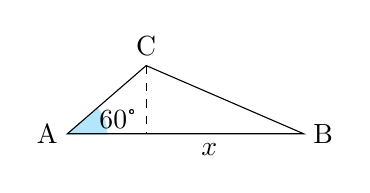
\begin{tikzpicture}
	\filldraw[cyan!30] (0,0) -- (0.5,0) arc(0:40:0.5) -- cycle;
	\draw (0,0) -- (3, 0)
	node[pos=0.6, below]{$x$}
	node[pos=1, right]{B} 
	-- (1,0.866) -- cycle
	node[pos=0, above]{C}
	node[pos=1, left]{A};
	\draw[dashed] (1,0.86)--++(0,-0.866)
	node[pos=0.5, below left]{60\textdegree	};
	\end{tikzpicture}
\end{center}
\divisor

La prima cosa da notare è il tipo di interferenza richiesto. Dato che viene chiesto quando un 
ascoltatore non sente più alcun suono, l'interferenza è distruttiva.\\
Per prima cosa però, è trovare la distanza $\overline{CB}$. Per fare ciò, poniamo $x$ la distanza
da B all'altezza.
\begin{equation*}
\overline{CB} = \sqrt{\sin(60)^2 + x^2} = \sqrt{\left(\frac{\sqrt{3}}{2}\right)^2 +
x^2} = \sqrt{\frac{3}{4} + x^2}
\end{equation*}
Il perché di questo è che $\sin(60)$ è l'altezza del triangolo e abbiamo posto $x$ come uno dei
cateti del triangolo rettangolo a destra.\\
Ora possiamo impostare la formula dell'interferenza distruttiva
\begin{align*}
\left\lvert \overline{PS}_1-\overline{PS}_2 \right\rvert = 
(2k + 1)\frac{\lambda}{2} \rightarrow \\
\sqrt{\frac{3}{4} + x^2} - 1 = \left(\frac{1}{2}+k\right)\cdot85
\end{align*}
Ora non resta che risolvere. Alla fine si dovrebbe arrivare ad un'equazione di questo genere
\begin{equation*}
x = \sqrt{18k^2 + 40k + 8.25}
\end{equation*}
Questa è un'equazione parametrica, nel parametro $k$. In questo caso assegnamo $k = 0$ in quanto il
testo chiede la \textbf{distanza minima} perché ci sia interferenza distruttiva. La prima frangia
distruttiva ha come $k$ il valore $0$. Terminando quindi
\begin{align*}
x = \sqrt{18k^2 + 40k + 8.25} \rightarrow \\
x = \sqrt{\cancel{18k^2} + \cancel{40k} + 8.25} \approx
\underline{2.87\,\text{m	}}
\end{align*}
Non è questo però il risultato finale. Il motivo è che $x$ non rappresenta completamente la
distanza tra A e B. Bisogna ancora aggiungere quella da A all'altezza. Quindi
\begin{equation*}
\overline{AB} = x + \cos(60) = 2.87 + 0.5 = \boxed{3.37\,\text{m}}
\end{equation*}

\subsubsection*{\hyperref[subsec:onde:young]{Esperienza di Young}}\label{ex:young}
\paragraph{Esercizio 1}
Nell'interferenza tra due fenditure poste a distanza $d = 25\,\text{cm}$ tra loro, si forma su uno 
schermo di distanza $l = 1\,\text{m}$ una figura il cui secondo massimo di intensità si trova ad $x = 
20\,\text{cm}$ dal massimo centrale. Calcola la \textbf{lunghezza d'onda dell'onda incidente}.
\divisor

Abbiamo come sempre varie strade per risolvere questo problema. La più facile è quella di invertire
la formula per trovare l'altezza di una frangia costruttiva. È costruttiva perché ci dice che è
\emph{il [\ldots] secondo massimo di intensità} che stiamo cercando. Quindi, invertiamo la formula
\begin{equation*}
y_n = \frac{l\cdot n\cdot\lambda}{d} \rightarrow \lambda = \frac{y_n\cdot d}{l\cdot n}
\end{equation*}
e semplicemente sostituiamo
\begin{equation*}
\lambda = \frac{y_n\cdot d}{l\cdot n} \rightarrow \lambda = \frac{0.2\cdot0.25}{1\cdot2} \rightarrow
\lambda = \boxed{0.025\,m} = \boxed{2.5\,\text{cm}}
\end{equation*}
Si noti che è stato posto $n=2$ in quanto chiede il secondo massimo.

\paragraph{Esercizio 2}
Nell'esperimento della doppia fenditura di Young, la prima frangia scura sopra la frangia centrale 
chiara appare ad un angolo di $\ang{0.29}$.\\
Calcola il \textbf{rapporto} tra la separazione delle fenditure $\boldsymbol{d}$ e la lunghezza 
d'onda della luce $\boldsymbol{\lambda}$.
\divisor

Per prima cosa, individuiamo la formula da usare. Abbiamo l'angolo e ci chiede $\dfrac{d}{\lambda}$.
Osservando che è una frangia scura, notiamo questa formula:
\begin{equation*}
\sin\theta_n = \left(n-\frac{1}{2}\right)\frac{\lambda}{d}
\end{equation*}
Notiamo che abbiamo tutto quello che ci serve per isolare $\dfrac{\lambda}{d}$ e poi farne il 
reciproco per ottenere quello che ci serve. Isolando quindi il risultato desiderato otteniamo
\begin{equation*}
\sin\theta_n = \left(n-\frac{1}{2}\right)\frac{\lambda}{d} \rightarrow
\frac{\sin\theta_n}{n-\frac{1}{2}} = \frac{\lambda}{d} \rightarrow
\frac{d}{\lambda} = \frac{n-\frac{1}{2}}{\sin\theta_n}
\end{equation*}
E ora non ci resta che inserire i valori
\begin{equation*}
\frac{d}{\lambda} = \frac{n-\frac{1}{2}}{\sin\theta_n} \rightarrow
\frac{d}{\lambda} = \frac{1-\frac{1}{2}}{\sin(0.29)} \rightarrow
\frac{d}{\lambda} \approx \frac{\frac{1}{2}}{0.005} \rightarrow
\frac{d}{\lambda} = \boxed{100}
\end{equation*}
Ovviamente con migliori approssimazioni si ottengono risultati più simili a $99$ ma un errore di
$1/100$ è accettabile.

\subsubsection*{\hyperref[subsec:onde:suono]{Suono}}\label{ex:suono}

\paragraph{Esercizio 1}
Due altoparlanti sono montati su una giostra di raggio $9.01\,\text{m}$. Quando la giostra è ferma, i 
due altoparlanti producono lo stesso suono alla frequenza di $100.0\,\text{Hz}$. Sono messi in 
posizione diametralmente opposta. La velocità del suono è $343.00\,\text{m/s}$ e la giostra fa un 
giro di $20.0\,\text{s}$. Qual è il \textbf{battimento} rilevato da un ascoltatore quando la giostra 
è posta in modo da avere gli altoparlanti paralleli all'ascoltatore?
\divisor

Come ricordiamo, la formula per i battimenti richiede due frequenze. Essendo che stiamo lavorando 
con il suono e la sorgente si muove, si usa Doppler.\\
Per prima cosa, troviamoci la velocità a cui ruota la giostra.
\begin{equation*}
v_t = \frac{2\pi r}{T} \rightarrow \frac{2\pi\cdot 9.01}{20} \approx \underline{2.83\,\text{m/s}}
\end{equation*}
Trovata la velocità, possiamo usare Doppler per trovare la frequenza percepita. Raddoppiamo il 
processo in quanto gli altoparlanti prima si avvicinano e poi si allontanano. Noi dobbiamo trovare
i battimenti prodotti da questo movimento.
\begin{equation*}
f = \frac{v + v_o}{v + v_s}\cdot f_s \rightarrow f = \frac{343+0}{343+2.83}\cdot 100
\approx\underline{99.19\,\text{Hz}}
\end{equation*}
\begin{equation*}
f = \frac{v + v_o}{v - v_s}\cdot f_s \rightarrow f = \frac{343+0}{343-2.83}\cdot 100
\approx\underline{100.83\,\text{Hz}}
\end{equation*}
In fine, usiamo i battimenti
\begin{equation*}
f_b = \left\vert f_o - f_s \right\vert \rightarrow f_b = \left\vert 100.83-99.19 \right\vert
\approx\boxed{1.64\,\text{Hz}}
\end{equation*}


\paragraph{Esercizio 2}
Una persona che si trova a $4.0\,m$ da una parte lancia un grido tale che il suono coplisce la 
parete con un'intensità di $2.5\cdot10^{-4}\,\text{W/m}^2$. Supponendo che la parete assorba il $20\%$
dell'energia sonora incidente e che rifletta il resto, qual è \textbf{il livello di intensità 
sonora} immediatamente prima e dopo che il suono è stato riflesso?
\divisor

Per prima cosa ci troviamo la superficie in cui il suono si diffonde. Dato che sappiamo il suono
si espande in forma sferica
\begin{equation*}
S = 4\pi r^2 \rightarrow S = 4\cdot16\pi \approx \underline{201.06\,\text{m}^2}
\end{equation*}
Avendo l'intensità e la superficie, possiamo trovarci l'energia semplicemente invertendo la formula
\begin{equation*}
I = \frac{E}{S} \rightarrow E = IS \rightarrow 2.5\cdot10^{-4}\cdot 201.06 \approx 
\underline{5.026\cdot10^{-2}\,\text{J}}
\end{equation*}
Questa è l'energia prima colpisca la parete, per trovare quella dopo
\begin{equation*}
20\%\cdot 5.026\cdot10^{-3} \approx 1\cdot10^{-3}\,\text{J}
\end{equation*}
e quindi l'$80\%$ equivale semplicemente a
\begin{equation*}
5.026\cdot10^{-4} - 1\cdot10^{-3} = \underline{4.026\cdot10^{-3}\,\text{J}}
\end{equation*}
Ci manca solo l'intensità nel secondo momento
\begin{equation*}
I = \frac{E}{S} \rightarrow I = \frac{4.026\cdot10^{-3}}{201.06} \approx
\underline{2\cdot10^{-5}\,\text{W/m}^2}
\end{equation*}
Ora abbiamo tutto quello che ci serve per finire l'esercizio. Ci troviamo dunque i livelli sonori
\begin{equation*}
L = 10\log_{10}\frac{I}{I_0} \rightarrow L_1 = 10\log_{10}\frac{2.5\cdot10^{-3}}{10^{-12}}
\approx\boxed{83.9\,\text{dB}}
\end{equation*}
\begin{equation*}
L = 10\log_{10}\frac{I}{I_0} \rightarrow L_2 = 10\log_{10}\frac{2\cdot10^{-5}}{10^{-12}}
\approx\boxed{83\,\text{dB}}
\end{equation*}

\subsubsection*{\hyperref[subsec:onde:lenti]{Lenti}}\label{ex:lenti}
\paragraph{Esercizio 1}
Due lenti sono disposte come in figura. Un fiammifero di altezza $2\,\text{cm}$ si trova a 
$5\,\text{cm}$ alla destra di una lente A che ha distanza focale $\overline{Af_A}$ pari a 
$3\,\text{cm}$. La seconda lente B, con una distanza focale $\overline{Bf_B}$ di $5\,\text{cm}$, 
deve essere posta a sinitra rispetto all'immaigne reale generata dalla prima, in maniera tale che 
essa formi un'immagine virtuale tre volte maggiore nei confronti dell'altezza del fiammifero vero e 
proprio. \textbf{Quale distanza separa le due lenti?}

\begin{center}
	\begin{tikzpicture}[scale=0.5]
		\coordinate (Cb) at (0,0);
		\coordinate (fb) at (2,0);
		\coordinate (fa) at (3,0);
		\coordinate (Ca) at (6,0);
		\coordinate (fa1) at (9,0);
		\coordinate (O) at (12,0);
		
		\draw ($(Cb) + (-0.5,0)$) -- ($(O) + (0.5,0)$);
		% Lenses
		\draw[<->] ($(Cb) + (0, -0.7)$) -- ($(Cb) + (0, 0.7)$)
			node[pos=1, above]{B};
		\draw[<->] ($(Ca) + (0, -0.7)$) -- ($(Ca) + (0, 0.7)$)
			node[pos=1, above]{A};
		\draw ($(fb) + (0, -0.3)$) -- ($(fb) + (0, 0.3)$)
			node[pos=1, above]{$f_B$};
		\draw ($(fa) + (0, -0.3)$) -- ($(fa) + (0, 0.3)$)
			node[pos=1, above]{$f_A$};
		\draw ($(fa1) + (0, -0.3)$) -- ($(fa1) + (0, 0.3)$)
			node[pos=1, above]{$f_A$};
		\draw ($(O) + (0, -0.5)$) -- ($(O) + (0, 0.5)$)
			node[pos=1, above]{Fiammifero};
 	\end{tikzpicture}
\end{center}
\divisor

Quest'esercizio non è facile e non è breve ma una volta risolto, si dovrebbe capire chiaramente come
risolvere altri esercizi sulle lenti.\\
Per prima cosa, si trovi la posizione dell'immagine nella prima riflessione
\begin{align*}
  \frac{1}{f} &= \frac{1}{q} + \frac{1}{f} \rightarrow
\frac{1}{q} = \frac{1}{f} - \frac{1}{p} \rightarrow\\
\frac{1}{q} &= \frac{1}{3} - \frac{1}{5} \rightarrow
\frac{1}{q} = \frac{2}{15} \rightarrow q = \underline{7.5\,\text{cm}}
\end{align*}
A questo punto, sapendo che deve essere ingrandita di tre volte ($G = 3$), possiamo usare la formula
dell'ingrandimento ed invertendola isolare $p$ per sapere la posizione dell'immagine e quindi sapere
la distanza tra le due lenti perché si ingrandisca tre volte. Possiamo farlo dato che la posizione 
dell'immagine della prima lente coincide con quella dell'oggetto della seconda lente.
\begin{equation*}
G = -\frac{q}{p} \rightarrow p = -\frac{q}{G} \rightarrow p = -\frac{q}{3}
\end{equation*}
La lasciamo in forma parametrica con il parametro $q$ in quanto è la nostra incognita.\\
Dato che ora stiamo lavorando con un'altra lente, riapplichiamo la prima formula
\begin{align*}
\frac{1}{f} = \frac{1}{q} + \frac{1}{f} \rightarrow
\frac{1}{5} = \frac{1}{-\frac{q}{3}} + \frac{1}{q} \rightarrow\\
\frac{1}{5} = -\frac{3}{q} + \frac{1}{q} \rightarrow
\frac{1}{5} = -\frac{2}{q} \rightarrow\\
\frac{q}{5} = -2 \rightarrow
q = \boxed{-10\,\text{cm}}
\end{align*}
Il risultato è negativo in quanto si trova dietro la prima lente, nostro punto di riferimento per
questo esercizio.

\subsection*{\hyperref[sec:elettrostatica]{Elettrostatica}}\label{ex:elettrostatica}
\paragraph{Esercizio 1}
Le armature di un condensatore piano hanno una superficie $S = 1\,m^2$ e distano $1\,\text{cm}$. Tra 
di loro c'è il vuoto. La differenza di potenziale applicata ai capi delle armature è $V = 
10^4\,\text{V}$. Calcolare la \textbf{capacità} del condesatore, la \textbf{carica} su ogni armatura, 
la \textbf{densità} di carica superficiale, l'\textbf{intensità} del campo elettrico.\\
Tra le armature del condensatore viene inserita una lamina di dielettrico di spessore $1\,\text{cm}$ 
e di costante elettrica relativa $\varepsilon_r = 5$. Calcolare la \textbf{densità} di carica 
superficiale, l'\textbf{intensità} del campo elettrico, la \textbf{d.d.p.} ai capi delle armature e 
la \textbf{capacità}.
\divisor

Questo esercizio è un esercizio direi riassuntivo di tutte le formule riguardanti i condensatori.
Per prima cosa possiamo immediatamente trovare la capacità del condensatore applicando una sola 
formula.
\begin{equation*}
C = \frac{S\varepsilon}{d} \rightarrow C = \frac{S\varepsilon_0}{d} \rightarrow 
C = \frac{1\cdot8.8\cdot10^{-12}}{0.01} = \boxed{8.8\cdot10^{-10}\,\text{F}}
\end{equation*}
E immediata viene anche la carica, invertendo la formula $C = \dfrac{Q}{V}$
\begin{equation*}
C = \frac{Q}{V} \rightarrow Q = C\cdot V \rightarrow Q = 8.8\cdot10^{-10}\cdot10^4 = 
\boxed{8.8\cdot\,\mu\text{C}}
\end{equation*}
La densità di carica ora viene immediata anch'essa
\begin{equation*}
\sigma = \frac{Q}{S} \rightarrow \sigma = \frac{8.8\cdot10{-6}}{1} = 
\boxed{8.8\cdot10^{-6}\,\text{C/m}^2}
\end{equation*}
E ora manca solo il campo elettrico, abbiamo due modi per trovarlo, questo è uno
\begin{equation*}
E = \frac{\Delta V}{\Delta x} \rightarrow \frac{10^4}{0.01} = \boxed{10^6\,\text{V/m}}
\end{equation*}
E questo era metà esercizio. Ora abbiamo lo stesso condensatore con un dielelettrico al suo interno.\\
La prima richiesta è la densità di carica. Risulta essere uguale a
\begin{equation*}
\sigma = \boxed{8.8\cdot10^{-6}\,\text{C/m}^2}
\end{equation*}
Ma è identica a prima? Come mai? Pensando un attimo, vediamo che il condensatore è isolato, quindi non
ci sono modi per cui le cariche si spostino. Essendo poi le due armature isolate fra di loro, la
carica non può spostarsi da una all'altra quindi la densità non varia.\\
Avendo chiarito questo punto, possiamo trovare l'intensità del campo elettrico
\begin{equation*}
E = \frac{\sigma}{\varepsilon} \rightarrow E = \frac{E_0}{\varepsilon_r} = 
\frac{10^6}{5} = \boxed{0.2\cdot10^{-6}\,\text{V/m}}
\end{equation*}
Qui abbiamo semplicemente scomposto la formula del campo elettrico:
\begin{equation*}
E = \frac{\sigma}{\varepsilon} \rightarrow E = \frac{\sigma}{\varepsilon_0\varepsilon_r} \rightarrow
E = \frac{\sigma}{\varepsilon}\cdot\frac{1}{\varepsilon_r} \rightarrow E = \frac{E_0}{\varepsilon_r}
\end{equation*}
E ora si trova la d.d.p.
\begin{equation*}
E = \frac{\Delta V}{\Delta x} \rightarrow \Delta V = E\Delta x \rightarrow 
\Delta V = 0.2\cdot10^{6}\cdot0.01 = \boxed{0.2\cdot10^{4}\,\text{V}}
\end{equation*}
Infine manca la capacità
\begin{align*}
C = \frac{\varepsilon S}{d} \rightarrow C =\frac{\varepsilon_0}{d}\varepsilon_r \rightarrow\\
C = C_0\varepsilon_r \rightarrow C = 8.8\cdot10^{-10}\cdot5 = \boxed{4.4\cdot10^{-9}\,\text{F}}
\end{align*}

\paragraph{Esercizio 2}
L'elettrone rappresentato in figura \textbf{è destinato a raggiungere l'armatura} del consdensatore 
caricata negativamente se questa dista $5\,\text{mm}$ dall'armatura positivamente? Se sì, determina 
con quale velocità, se no, determina quale avrebbe dovuto essere la velocità iniziale minima in grado 
di consentirgli di raggiungere l'armatura.
\begin{itemize}
	\item $v_0 = 750\,\text{m/s}$
	\item $\text{E} = 3.5\cdot10^{-4}\,\text{N/C}$
\end{itemize}
\begin{center}
	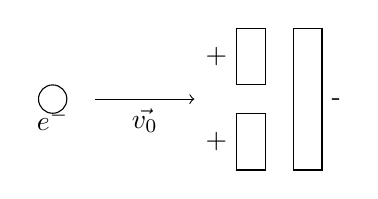
\begin{tikzpicture}[scale=1.8]
		\draw (0,0) circle (0.1)
			node[below]{$\text{e}^{-}$};
		\draw[->] (0.3, 0) -- ++(0.7, 0)
			node[pos=0.5, below]{$\vec{v_0}$};
		\draw (1.3,0.5) -- (1.3,0.1) node[pos=0.5,left]{+} -- (1.5,0.1) -- (1.5,0.5) -- cycle;
		\draw (1.3,-0.5) -- (1.3,-0.1) node[pos=0.5,left]{+} -- (1.5,-0.1) -- (1.5,-0.5) -- cycle;
		\draw (1.7,0.5) -- (1.7,-0.5) -- (1.9,-0.5) -- (1.9,0.5) node[pos=0.5,right]{-} -- cycle;
	\end{tikzpicture}
\end{center}
\divisor

Allora, per prima cosa vediamo da che parte il campo elettrico va: dato che le cariche positive sono a
sinistra, il campo segue questo verso ed è in linea con la velocità. Poi però notiamo che appena 
l'elettrone entra nel condensatore subirà una forza contraria in quanto ha carica negativa così come 
l'armatura di destra.\\[\baselineskip]

Chiariti questi punti, come possiamo sapere se arriverà alla seconda armatura? Una formula molto 
comoda del modo rettilineo uniformemente accelerato torna utile:
\begin{equation*}
v_f^2 - v_i^2 = 2aS
\end{equation*}
Con questa possiamo sapere quanta distanza percorre il nostro elettrone. Se è inferiore alla distanza
tra le armature, allora la velocità non è sufficiente. Ora il problema è: come troviamo 
l'accelerazione? Ci tocca invertire la formula fondamentale della dinamica
\begin{equation*}
\vec{F} = m\vec{a} \rightarrow \vec{a} = \frac{\vec{F}}{m}
\end{equation*}
ma il problema è: qual è la forza? Ovviamente è quella repulsiva che l'elettrone sente a causa 
dell'armatura caricata negativamente. Come trovarla? Semplice
\begin{equation*}
\vec{F} = q\vec{E} \rightarrow F = qE = -1.60\cdot10^{-19}\cdot3.5\cdot10^{-4} = 
\underline{-5.6\cdot10^{-23}\,\text{N}}
\end{equation*}
E ora possiamo trovare l'accelerazione
\begin{equation*}
a = \frac{F}{m} \rightarrow a = \frac{-5.6\cdot10^{-23}}{9.11\cdot10^{-28}} = 
\underline{-6.1\cdot10^4}
\end{equation*}
Ora completiamo l'equazione precedente
\begin{equation*}
v_f^2 - v_i^2 = 2aS \rightarrow S = \frac{v_f^2 - v_i^2}{2a} \rightarrow 
S = \frac{0^2 - 750^2}{2\cdot6.1\cdot10^4} = \boxed{4.5\,\text{mm}}
\end{equation*}
Essendo questa distanza inferiore a $5\,\text{mm}$, l'elettrone non raggiungerà l'altra armatura.\\
Seguendo lo stesso ragionamento invertiamo questa formula per trovare $v_i$ sapendo la distanza.
\begin{align*}
v_f^2 - v_i^2 = 2aS \rightarrow v_i = \sqrt{2aS + v_f^2} \rightarrow \\
v_i = \sqrt{2\cdot6.1\cdot10^4\cdot5} \approx \boxed{784\,\text{m/s}}
\end{align*}

\paragraph{Esercizio 3}
Un elettrone di massa $m$ e carica $e$ viene lanciato ad una velocità $v_0=2\cdot10^8\,\text{m/s}$
lungo l'asse delle pareti di un condensatore a facce piane e parallele di lunghezza $l=1\,\text{m}
$, andando a colpire uno schermo fluorescente posto ad una distanza $d=2\,\text{m}$ dagli etremi 
delle pareti del condensatore. Supponendo che l'eltrrone appena uscito dal condensatore non
risenta più dell'effetto del campo elettrico e che il campo elettrico $\vec{E}$, di modulo
$10^4\,\text{N/C}$, sia diretto verso il basso, \textbf{calcola a quale distanza dall'asse del
condensatore, l'elettrone colpisce lo schermo.} Si tenga presente che 
$\frac{e}{m}=1.76\cdot10^{11}\,\text{C/kg}$
\divisor

Quest'esercizio è piuttosto complicato ed è molto articolato. Andrà a toccare elementi di 
cinematica nonché di elettrostatica. Per avere un'idea più chiara della situazione, andiamo a 
vedere il disegno

\begin{center}
  \begin{tikzpicture}
    \coordinate (C1) at (0,0);
    \coordinate (C2) at (2,0);
    \coordinate (C3) at (0,1);
    \coordinate (C4) at (2,1);

    \coordinate (Start) at (0,0.5);
    \coordinate (End1) at (2,0.9);
    \coordinate (End2) at (6,2.5);

    \coordinate (H) at (6,0.5);
    \coordinate (L) at (6,0.9);

    \draw (C1) -- (C2);
    \draw (C3) -- (C4);

    \draw[thick, red, -stealth] (Start) to[out=2, in=200] (End1);
    \draw[dashed] (Start) -- ++(6,0);
    \draw[dashed] (End1) -- ++(4,0);
    \draw[thick, red, -stealth] (End1) -- (End2);

    \draw (6,3) -- ++(0,-3);

    \foreach \x in {0.5, 1, 1.5}{
      \draw[lightgray, -stealth] (\x, 1) -- (\x, 0);
    }

    \draw[|-|] ($(End2) + (0.1,0)$) -- ($(H) + (0.1,0)$)
      node[pos=0.5,right]{$d$};
    \draw[|-|] ($(L) + (0.4,0)$) -- ($(H) + (0.4,0)$)
      node[pos=0.5,right]{$y_{usc}$};
    \markangle{End1}{End2}{L}{0.8}{1.2}{$\alpha$}
  \end{tikzpicture}
\end{center}

In rosso vediamo il moto dell'elettrone. Perché tende verso l'alto? L'elettrone ha carica
negativa, il campo elettrico va da + a -, quindi l'elettrone si muove in verso opposto a
quello del campo. Sono stati evidenziati anche i due diversi moti, con due diverse frecce.
Il primo è moto parabolico in quanto abbiamo una certa forza che agisce sull'elettrone, il secondo
è moto rettilineo uniforme in quanto non ci sono più forze in gioco.\\ [\baselineskip]
Per risolvere questo genere di esercizi molto articolati, bisogna procedere con calma e metodo.
Noi dobbiamo trovare $d$. $d$ è composta da $y_{usc}$ e dalla $y$ del moto rettilineo. Troviamo
intanto $y_{usc}$. Secondo la legge oraria del moto parabolico
\begin{equation*}
  y_{usc} = \frac{1}{2}at^2 \rightarrow y_{usc} = \frac{1}{2}a \left( \frac{x}{v_0} \right)^2
\end{equation*}
Abbiamo tutto quello che ci serve tranne $a$. A che accelerazione è sottoposto l'elettrone?
A quella generata dalla forza di un campo magnetico su una carica. Utilizzando quindi la 
definizione di campo elettrico e la seconda legge della dinamica scriviamo
\begin{equation*}
  eE = ma \rightarrow a = \frac{e}{m}E
\end{equation*}
Quindi sostituendo con i dati già forniti e risolvendo otteniamo
\begin{equation*}
  a \approx \underline{1.76\cdot10^{15}\,\text{m/s}^2} 
\end{equation*}
Inserendo ora tutti i dati nella prima formula
\begin{equation*}
  y_{usc} = \frac{1}{2}\cdot1.76\cdot10^5\cdot \left( \frac{1}{2\cdot10^8} \right)^2
  \approx \underline{2.2\cdot10^{-2}\,\text{m}} 
\end{equation*}
E questa era la parte facile. Ora se osserviamo meglio il disegno, vediamo che $y=2\tan\alpha$
questo perché $2$ è il cateto maggiore e $\alpha$ l'angolo opposto al cateto che ci interessa.
Quindi dobbiamo in qualche modo trovare $\alpha$. Possiamo vedere quell'angolo come angolo 
compreso tra due vettori, specificamente la componente $x$ e $y$ della velocità d'uscita.
Abbiamo già la componente $x$ in quanto nel moto parabolico si mantiene costante. Quella
$y$ è facilmente trovabile con le nostre conoscenze di cinematica dove
\begin{equation*}
  v=v_0+at
\end{equation*}
dove $v_0=0$ in quanto l'elettrone parte da fermo sull'asse $y$. L'accelerazione e il tempo li
abbiamo già individuati! Quindi scriviamo
\begin{equation*}
  v=at \rightarrow v=1.76\cdot10^{15}\cdot\frac{1}{2\cdot10^8}\approx
  \underline{8.8\cdot10^6\,\text{m/s}} 
\end{equation*}
L'angolo compreso tra due vettori è pari all'arcotangente del quoziente tra le componenti $y$ e
$x$. Quindi
\begin{equation*}
  \alpha=\arctan \frac{y}{x} \rightarrow \alpha=\arctan \frac{8.8\cdot10^6}{2\cdot10^8}\approx 
  \underline{2.5\text{\textdegree}} 
\end{equation*}
Ora risolviamo e concludiamo
\begin{align*}
  d &= y+y_{usc} = 2\tan\alpha+y_{usc} = 2\tan2.5+0.022 =\\
    &2\cdot0.044+0.022 = \boxed{0.11\,\text{m}}
\end{align*}

\subsection*{\hyperref[sec:circElettr]{Circuiti Elettrici}}\label{ex:circElettr}
\paragraph{Esercizio 1}
Se la corrente nel resistore di $6\,\Omega$ della figura è di $2\,A$:
\begin{itemize}[label={$\bullet$}]
	\item La caduta di potenziale tra a e b;
	\item La corrente totale del circuito;
\end{itemize}
\begin{center}
	\ctikzset{bipoles/length=.8cm}
	\begin{circuitikz}
		\draw 
		(-1,0) node[above]{a}
		to [short, o-] (0,0)
		to [short, *-] (0,1)
		to [short] (1,1)
		to [R, l=10<\ohm>] (2,1)
		to [short] (3,1)
		to [R, l=6<\ohm>] (4,1)
		to [short] (4.5,1)
		to [short] (4.5,0)
		
		(0,0) 
		to [short, *-] (0,-1)
		to [short] (0.5,-1)
		to [short] (0.5,-0.5)
		to [short] (1, -0.5)
		to [R, l=8<\ohm>] (2,-0.5)
		to [short] (2.5,-0.5)
		to [short] (2.5,-1)
		(0.5,-1)
		to [short] (0.5,-1.5)
		to [short] (1,-1.5)
		to [R, l=8<\ohm>] (2,-1.5)
		to [short] (2.5,-1.5)
		to [short] (2.5,-1)
		
		(2.5,-1)
		to [short] (3,-1)
		to [R, l=8<\ohm>] (4,-1)
		to [short] (4.5,-1)
		to [short] (4.5,0);
		
		\draw(4.5,0)
		to [short, *-o] (5.5,0) node[above]{b};
	\end{circuitikz}
\end{center}
\divisor

Per prima cosa, si semplifichino le resistenze da $8\,\Omega$ che sono in parallelo fra di loro
\begin{equation*}
\frac{1}{R_e} = \frac{1}{R_1} + \frac{1}{R_2} \rightarrow
\frac{1}{R_e} = \frac{1}{8} + \frac{1}{8} \rightarrow
R_e = \underline{4\,\Omega}
\end{equation*}

Quindi ora il circuito è come questo
\begin{center}
	\ctikzset{bipoles/length=.8cm}
	\begin{circuitikz}
		\draw 
		(-1,0) node[above]{a}
		to [short, o-] (0,0)
		to [short, *-] (0,1)
		to [short] (1,1)
		to [R, l=10<\ohm>] (2,1)
		to [short] (3,1)
		to [R, l=6<\ohm>] (4,1)
		to [short] (4.5,1)
		to [short] (4.5,0)
		
		(0,0) 
		to [short, *-] (0,-1)
		to [short] (1,-1)
		to [R, l=4<\ohm>] (2,-1)
		to [short] (3,-1)
		to [R, l=8<\ohm>] (4,-1)
		to [short] (4.5,-1)
		to [short] (4.5,0);
		
		\draw(4.5,0)
		to [short, *-o] (5.5,0) node[above]{b};
	\end{circuitikz}
\end{center}

Semplifichiamolo ulterirormente riducendo le resistenze in serie
\begin{equation*}
R_{e_1} = 10 + 6 = \underline{16\,\Omega}
\end{equation*}
\begin{equation*}
R_{e_2} = 4 + 8 = \underline{12\,\Omega}
\end{equation*}

E il circuito ora rimane molto semplicemente
\begin{center}
	\ctikzset{bipoles/length=.8cm}
	\begin{circuitikz}
		\draw
		(-1,0) node[above]{a}
		to [short, o-] (0,0)
		to [short, *-] (0,1)
		to [short] (1,1)
		to [R, l=16<\ohm>] (2,1)
		to [short] (3,1)
		to [short, -*] (3,0);
		
		\draw
		(0,0)
		to [short, *-] (0,-1)
		to [short] (1,-1)
		to [R, l=12<\ohm>] (2,-1)
		to [short] (3,-1)
		to [short, -*] (3,0)
		to [short, -o] (4,0) node[above]{b};
	\end{circuitikz}
\end{center}

Sapevamo che nella resistenza da $6\,\Omega$ del primo circuito passvano $2\,A$. Dato che si trova 
in serie con una da $10\,\Omega$, anche in questa passeranno $2\,A$.\\
Sfruttando la formula
\begin{equation*}
V = Ri
\end{equation*}
possiamo trovarci la caduta di potenziale tra a e b.
\begin{equation*}
V = Ri \rightarrow V = 16\cdot2 = \boxed{32\,\text{V}}
\end{equation*}

Sapendo ora la d.d.p.~e sapendo che le resistenze sono in parallelo, possiamo trovarci la corrente
che passa nella resistenza di $12\,\Omega$ invertendo quella formula
\begin{equation*}
V = Ri \rightarrow i = \frac{V}{R} \rightarrow i = \frac{32}{12} \approx \underline{2.66\,\text{V}}
\end{equation*}

Infine, la sommiamo alla corrente del ramo "superiore" del circuito e otteniamo la corrente totale
\begin{equation*}
i_t = i_1 + i+2 = 2 + 2.66 = \boxed{4.66\,\text{A}}
\end{equation*}

\paragraph{Esercizio 2}
Calcolare la resistenza $R_{eq}$ vista ai morsetti \textbf{A-B}
\begin{multicols}{2}
	\begin{itemize}
		\item $R_1 = R_3 = 0.2\,\Omega$
		\item $R_2 = 0.4\,\Omega$
		\item $R_4 = R_5 = 1\,\Omega$
		\item $R_6 =3\,\Omega$
	\end{itemize}
\end{multicols}

\begin{center}
	\ctikzset{bipoles/length=1cm}
	\begin{circuitikz}[scale=1.9]
		\draw (1,0) to[R=$R_1$, -*] (1,1) node[above]{A} % A
		to[R=$R_2$, -*] (2,1) node[above]{C}
		to[R=$R_5$] (3,1)
		to[R=$R_6$] (3,0)
		to[short, -*] (2,0) node[below]{D}
		to[short, -*] (1,0) node[below]{B};
		\draw (2,1) to[R=$R_3$] (1,0);
		\draw (2,1) to[R=$R_4$] (2,0);
	\end{circuitikz}
\end{center}
\divisor

Quest'esercizio, per quanto apparentemente intimidatorio, non è così complicato. La prima cosa da fare
è trovare in che relazione sono le resistenze fra di loro. È immediato vedere che $R_5$ e $R_6$ sono
in serie fra di loro in quanto non hanno collegamenti nel mezzo.\\
E ora come scoprire i collegamenti di quell'aggroviglio di resistenze? Bisogna andare con molta calma
e osservare come si diffonde la corrente. Sappiamo che A e B sono i poli della batteria quindi 
ipotizziamo che in A si trovi il polo positivo (metterlo in B non cambierebbe nulla). Il seguente
schema chiarisce i versi delle correnti.
\begin{center}
	\ctikzset{bipoles/length=1cm}
	\begin{circuitikz}[scale=1.9]
		\draw (1,0) to[R=$R_1$, i^=$i_4$, -*] (1,1) node[above]{A} % A
		to[R=$R_2$, i^=$i$, -*] (2,1) node[above]{C}
		to[R=$R_5$, i^=$i_1$] (3,1)
		to[R=$R_6$, i^=$i_1$] (3,0)
		to[short, -*] (2,0) node[below]{D}
		to[short, -*] (1,0) node[below]{B};
		\draw (2,1) to[R=$R_3$, i^=$i_2$] (1,0);
		\draw (2,1) to[R=$R_4$, i^=$i_3$] (2,0);
	\end{circuitikz}
\end{center}
Come possiamo notare in C la corrente si divide in 3: $i_1$, $i_2$ e $i_3$. Questo cosa ci dice? Che i
tre collegamenti sono fra di loro in parallelo! Una proprietà dei collegamenti in serie è che la 
corrente si mantiene costante tra le resistenze, dato che in questo caso non avviene il collegamento
è in parallelo.\\
Abbiamo quindi definito che $R_5$ ed $R_6$ sono in serie fra di loro; la loro equivalente, $R_4$ ed
$R_3$ sono in parallelo fra di loro. Manca solo $R_1$ ed $R_2$. $R_2$ è immediatamente visibile che 
sarà in serie con la risultante di $R_5$, $R_6$, $R_4$ ed $R_3$. Quando rimarranno solo due 
resistenze, $R_1$ e l'altra saranno in parallelo.\\[\baselineskip]

Per rendere tutto più chiaro, cominciamo a fare i calcoli e semplificare il circuito.
\begin{equation*}
R_{5/6} = R_5 + R_6 \rightarrow R_{5/6} = 1 + 3 = \underline{4\,\Omega}
\end{equation*}

\begin{center}
	\ctikzset{bipoles/length=1cm}
	\begin{circuitikz}[scale=1.9]
		\draw (1,0) to[R=$R_1$, i^=$i_4$, -*] (1,1) node[above]{A} % A
		to[R=$R_2$, i^=$i$, -*] (2,1) node[above]{C}
		to[short] (3,1)
		to[R=$R_{5/6}$, i^=$i_5$] (3,0)
		to[short, -*] (2,0) node[below]{D}
		to[short, -*] (1,0) node[below]{B};
		\draw (2,1) to[R=$R_3$, i^=$i_2$] (1,0);
		\draw (2,1) to[R=$R_4$, i^=$i_3$] (2,0);
	\end{circuitikz}
\end{center}
Avendo già stabilito il verso di percorrenza della corrente e i tipi di collegamento, semplifichiamo
$R_{5/6}$, $R_4$ e $R_3$.
\begin{align*}
R_{3/4/5/6} = \left(\frac{1}{R_3} + \frac{1}{R_4} + \frac{1}{R_{5/6}}\right)^{-1} \rightarrow\\
\left(\frac{1}{0.2} + \frac{1}{1} + \frac{1}{4}\right)^{-1} = \underline{0.16\,\Omega}
\end{align*}

\begin{center}
	\ctikzset{bipoles/length=1cm}
	\begin{circuitikz}[scale=1.9]
		\draw (1,0) to[R=$R_1$, i^=$i_4$, -*] (1,1) node[above]{A} % A
		to[R=$R_2$, i^=$i$, -*] (2,1) node[above]{C}
		to[R=$R_{3/4/5/6}$, i^=$i$, -*] (2,0) node[below]{D}
		to[short, -*] (1,0) node[below]{B};
	\end{circuitikz}
\end{center}
Ora semplifichiamo le due resistenze in serie ($R_2$ e l'ultima calcolata)
\begin{align*}
R_{2/3/4/5/6} = R_2 + R_{3/4/5/6} \rightarrow \\
R_{2/3/4/5/6} = 0.4 + 0.16 = \underline{ 0.56\,\Omega}
\end{align*}

\begin{center}
	\ctikzset{bipoles/length=1cm}
	\begin{circuitikz}[scale=1.9]
		\draw (0.5,0) to[R=$R_1$, i^=$i_4$] (0.5,1)
		to[short, -*] (1,1) node[above]{A} % A
		to[short] (1.5,1)
		to[R=$R_{2/3/4/5/6}$, i^=$i$] (1.5,0)
		to[short, -*] (1,0) node[below]{B}
		to[short] (0.5,0);
	\end{circuitikz}
\end{center}
E ora possiamo vedere che le due resistenze sono in parallelo fra di loro e quindi possiamo
semplificarle con facilità
\begin{align*}
R_{eq} = \left(\frac{1}{R_1} + \frac{1}{R_{2/3/4/5/6}}\right)^{-1} \rightarrow\\
R_{eq} = \left(\frac{1}{0.2} + \frac{1}{0.56}\right)^{-1} = \boxed{0.147\,\Omega}
\end{align*}
Ed ecco il nostro risultato. Il modo migliore per risolvere questi esercizi è cercare di capire
in che verso va la corrente e vedere i collegamenti. Andando con calma si riuscirà senza problemi a 
risolvere qualsiasi esercizio proposto.

\paragraph{Esercizio 3}
Per la disposizione mostrata in figura si trovino:
\begin{itemize}[label={$\bullet$}]
	\item La capacità equivalente tra i terminali
	\item La carica immagazzinata in ciascun condensatore
	\item L'energia accumulata nei condensatori
\end{itemize}
\begin{center}
		\ctikzset{bipoles/length=1cm}
	\begin{circuitikz}
		\draw (0,0) to[short, o-] (3,0)
		to[short] (4,0)
		to[C, l_=12<\micro\farad>] (4,2)
		to[short] (4,2)
		to[short, -o] (0,2);
		\draw (2,0) to[C=4<\micro\farad>] (2,1)
		to[C=15<\micro\farad>] (2,2);
		\path node[above] (0,1) {$200\,\text{V}$};
	\end{circuitikz}
\end{center}
\divisor

È evidente che i due condesatori da $15$ e $4$ sono in serie fra di loro. Il condesatore da $12$ 
invece è in parallelo con questi due. Per risolvere il primo punto calcoliamoci l'equivalente dei
due condensatori in serie.
\begin{equation*}
\frac{1}{C_{eq}} = \frac{1}{C_1} + \frac{1}{C_2} \rightarrow
C_{eq} = \left(\frac{1}{15} + \frac{1}{4}\right)^{-1} \approx\underline{3.15\,\text{pF}}
\end{equation*}
Ora il circuito è come questo
\begin{center}
	\ctikzset{bipoles/length=1cm}
	\begin{circuitikz}
		\draw (0,0) to[short, o-] (1,0)
		to[short] (2,0)
		to[C, l_=12<\micro\farad>] (2,2)
		to[short] (2,2)
		to[short, -o] (0,2);
		\draw (1,0) to[C=3.15<\micro\farad>] (1,2);
	\end{circuitikz}
\end{center}
Ora basta solo trovare l'equivalente di questi due in parallelo.
\begin{equation*}
C_{eq} = C_1 + C_2 \rightarrow 3.15 + 12 = \boxed{15.15\,\text{pF}}
\end{equation*}

Per il secondo punto possiamo sfruttare la formula per la capacità elettrica $C = \dfrac{Q}{V}$. Dato
che i due condensatori dell'ultimo circuito sono in parallelo fra di loro, la d.d.p.~rimane uguale. 
Quindi possiamo invertire la formula e trovare immediatamente la carica nel condesatore da 12.
\begin{equation*}
C = \frac{Q}{V} \rightarrow Q = C\cdot V \rightarrow Q = 12\cdot10^{-6}\cdot200 =
\boxed{2400\,\mu\text{C}}
\end{equation*}
E possiamo fare lo stesso con la resistenza equivalente. Una volta fatto otterremo anche la carica su 
ciascuno dei due condensatori in quanto sono in serie e due condensatori in serie hanno la stessa 
carica.
\begin{equation*}
C = \frac{Q}{V} \rightarrow Q = C\cdot V \rightarrow Q = 3.15\cdot200 = \boxed{630\,\mu\text{C}}
\end{equation*}

\paragraph{Esercizio 4}
Un sottile filo conduttore di resistenza $R = 50\Omega$, collegato ad un generatore di tensione
ideale che mantiene una differenza di potenziale $\Delta V_0$, viene utilizzato per portare
$10$L di acqua dalla temperatura di $10$\textdegree a quella di $50$\textdegree. La corrente
erogata dal generatore è pari a $5$A. Considera il calore specifico dell'acqua pari a 
$4186$ J/kg$\cdot$K e il rendimento del sistema pari a $\mu=0.8$
\divisor

In questo esercizio combiniamo le nostre conoscenze di Calorimetria e di elettrostatica. Abbiamo
una resistenza che è attraversata da una corrente. Questo ci dice, secondo l'effetto Joule che 
si scalderà. Scaldandosi emetterà calore anche ai corpi adiacenti, in questo caso l'acqua.\\
Sapendo che per Joule
\begin{equation*}
  Q = Ri^2t
\end{equation*}
e che la quantità di calore è pari a
\begin{equation*}
  Q = C\Delta t = mc\Delta T
\end{equation*}
unendole otteniamo
\begin{equation*}
  Ri^2t\cdot = C= mc\Delta T\mu
\end{equation*}
Abbiamo aggiunto $\mu$ in quanto la macchina termica non è perfetta e ha un rendimento diverso da 
1. Dato che a noi interessa solo il tempo, lo isoliamo per ottenere
\begin{equation*}
  t = \frac{mc\Delta T}{Ri^2} 
\end{equation*}
Ora non resta che sostituire
\begin{equation*}
t = \frac{mc\Delta T\mu}{Ri^2} \rightarrow t =  \frac{10\cdot4186\cdot(50-10)\cdot0.8}{50\cdot5^2}
= \boxed{1.7\cdot10^3\,\text{s}}
\end{equation*}

\paragraph{Esercizio 5}
Un generatore di forza elettromotrice pari a $\mathcal{E} = 30\,\text{V}$ è connesso in serie ad
una resistenza $R=5\,\text{k}\Omega$ e ad un condensatore di capacità pari a $8\,\mu\text{F}$.
Un interruttore chiude il circuito all'istante $t=0\,\text{s}$. Calcola quante \textbf{costanti di
tempo siano necessarie perché l'energia immagazzinata sia $\frac{1}{3}$ dell'energia finale.}\\ 
L'energia immagazzinata in un condensatore in funzione del tempo è
\begin{equation*}
  L_c(t) = \frac{q(t)^2}{2C}
\end{equation*}
\divisor

Partiamo dal disegno del circuito
\begin{center}
  \ctikzset{bipoles/length=1cm}
  \begin{circuitikz}
    \draw (0,0) 
      to[battery1] (0,1)
      to[R] (3,1)
      to[C] (3,0)
      to[switch] (0,0);
  \end{circuitikz}
\end{center}

Ora, osservando la formula che ci viene data, possiamo riscriverla
\begin{equation*}
  L_c(t) = \frac{q(t^2)}{2C} = \frac{1}{2}q(t)V(t)
\end{equation*}
che ulteriormente espansa e semplificata viene
\begin{equation*}
  L_c(t) = \underbrace{\frac{1}{2}C\mathcal{E}^2}_{\text{max}} \left( 1-e^{-\frac{t}{\tau}} \right)^2 
\end{equation*}
Dato che noi dobbiamo ottenere $\frac{1}{3}$ della capacità massima, possiamo scrivere la
seguente equazione
\begin{align*}
  \frac{1}{2}\frac{1}{3}C\mathcal{E}^2 &= \frac{1}{2}C\mathcal{E}^2 \left( 1-e^{-\frac{t}{\tau}} \right)^2 \rightarrow \\
  \sqrt{\frac{1}{3}} &= \sqrt{\left( 1-e^{-\frac{t}{\tau}} \right)^2} \rightarrow \\
  0.42 &= e^{-\frac{t}{\tau}} \rightarrow \ln0.42 = -\frac{t}{\tau} \rightarrow \\
  t &\approx\boxed{0.86\tau}
\end{align*}
\subsection*{\hyperref[sec:magnetismo]{Magnetismo}}\label{ex:magnetismo}
\paragraph{Esercizio 1}
Tre fili rettilinei paralleli sono posti sui vertici di un triangolo equilatero di lato 
$d=35\,\text{cm}$, come mostrato in figura e sono attraversati dalle correnti $i_1$, $i_2$, $i_3$. Le
correnti hanno tutte intensità pari a $2\,\text{A}$. \textbf{Determina modulo, direzione e verso
della forza per unità di lunghezza che agisce su un punto al centro del triangolo nel caso in cui
tutte le correnti siano uscenti dal foglio. E se uno fosse entrante?}
\divisor

\begin{center}
	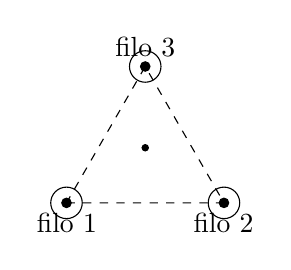
\begin{tikzpicture}[scale=2]
		\draw[dashed] (0,0) coordinate (A) --+(1,0) coordinate (B) --+(60:1) coordinate (C) -- cycle;
		\filldraw (A) circle (0.03);
		\filldraw (B) circle (0.03);
		\filldraw (C) circle (0.03);
		\draw (A) circle (0.1)
			node[xshift=-0.5cm,yshift=-0.5cm,anchor=south west]{filo $1$};
		\draw (B) circle (0.1)
			node[xshift=0.5cm,yshift=-0.5cm,anchor=south east]{filo $2$};
		\draw (C) circle (0.1)
			node[yshift=0.5cm,anchor=north]{filo $3$};
		\filldraw (0.5,0.35) circle (0.02);
	\end{tikzpicture}
\end{center}
Questo è il nostro disegno e il punto al centro è quello su cui noi dobbiamo trovare la forza 
risultante. Scriviamo la formula per la forza che intercorre tra due fili paralleli (legge di Ampére)
\begin{equation*}
F = \frac{\mu_0}{2\pi}\frac{i_1i_2}{d}l
\end{equation*}
sappiamo però che tutte le correnti sono uguali quindi semplifichiamo in
\begin{equation*}
F = \frac{4l\mu_0}{2d\pi}
\end{equation*}
Abbiamo $d$ che rappresenta la distanza tra i due punti e $l$ che è un parametro variabile. Usando la
\hyperref[subsec:vettori:prodottoVettoriale]{regola della mano} troviamo la direzione e il verso dei
vettori.
\begin{center}
	\begin{tikzpicture}[scale=2]
		\draw[dashed] (0,0) coordinate (A) --+(1,0) coordinate (B) --+(60:1) coordinate (C) -- cycle;
		\filldraw (A) circle (0.03);
		\filldraw (B) circle (0.03);
		\filldraw (C) circle (0.03);
		\draw (A) circle (0.1)
			node[xshift=-0.5cm,yshift=-0.5cm,anchor=south west]{filo $1$};
		\draw (B) circle (0.1)
			node[xshift=0.5cm,yshift=-0.5cm,anchor=south east]{filo $2$};
		\draw (C) circle (0.1)
			node[yshift=0.5cm,anchor=north]{filo $3$};
		\filldraw (0.5,0.28) coordinate (O) circle (0.02);
		\draw[-stealth] (O) -- ($(A)!.5!(B)$);
		\draw[-stealth] (O) -- ($(A)!.5!(C)$);
		\draw[-stealth] (O) -- ($(C)!.5!(B)$);
	\end{tikzpicture}
\end{center}
Quello che capiamo da questo disegno è decisivo: le tre forze si annullano se hanno lo stesso modulo.
Come mai? Ipotiziamo di proiettare su $x$ e $y$ le componenti
\begin{center}
	\begin{tikzpicture}[scale=2]
		\draw[dashed] (0,0) coordinate (A) --+(1,0) coordinate (B) --+(60:1) coordinate (C) -- cycle;
		\filldraw (A) circle (0.03);
		\filldraw (B) circle (0.03);
		\filldraw (C) circle (0.03);
		\draw (A) circle (0.1)
			node[xshift=-0.5cm,yshift=-0.5cm,anchor=south west]{filo $1$};
		\draw (B) circle (0.1)
			node[xshift=0.5cm,yshift=-0.5cm,anchor=south east]{filo $2$};
		\draw (C) circle (0.1)
			node[yshift=0.5cm,anchor=north]{filo $3$};
		\filldraw (0.5,0.28) coordinate (O) circle (0.02);
		\draw[-stealth] (O) -- ($(A)!.5!(B)$);
		\draw[-stealth] (O) -- ($(A)!.5!(C)$);
		\draw[-stealth] (O) -- ($(C)!.5!(B)$);
		\draw[densely dotted] (0,0.28) -- (1,0.28);
		\coordinate (M1) at ($(A)!.5!(B)$);
		\coordinate (M2) at ($(A)!.5!(C)$);
		\coordinate (M3) at ($(C)!.5!(B)$);
		\coordinate (R) at (0,0.28);
		\draw[red, thick] (M2 |- R) -- (O);
		\draw[red, thick] (M3 |- R) -- (O);
		\draw[red, thick] (O |- M2) -- (O);
	\end{tikzpicture}
\end{center}
Notiamo che la coponente $x$ si annulla e quella $y$ perché bisogna sommare le due componenti dei 
vettori. Di conseguenza
\begin{equation*}
\vec{F} = \vec{0}
\end{equation*}
E se uno fosse entrante? Ipotiziamo che quello entrante sia il filo $1$. Il disegno dei vettori ora 
diventa
\begin{center}
	\begin{tikzpicture}[scale=2]
		\draw[dashed] (0,0) coordinate (A) --+(1,0) coordinate (B) --+(60:1) coordinate (C) -- cycle;
		\filldraw (A) circle (0.03);
		\filldraw (B) circle (0.03);
		\filldraw (C) circle (0.03);
		\draw (A) circle (0.1)
			node[xshift=-0.5cm,yshift=-0.5cm,anchor=south west]{filo $1$};
		\draw (B) circle (0.1)
			node[xshift=0.5cm,yshift=-0.5cm,anchor=south east]{filo $2$};
		\draw (C) circle (0.1)
			node[yshift=0.5cm,anchor=north]{filo $3$};
		\filldraw (0.5,0.28) coordinate (O) circle (0.02);
		\draw[-stealth] (O) -- ($(A)!.5!(B)$);
		\draw[-stealth] (O) -- ($(C)!.5!(B)$);
		
		\coordinate (M1) at ($(A)!.5!(B)$);
		\coordinate (M2) at ($(A)!.5!(C)$);
		\coordinate (M3) at ($(C)!.5!(B)$);
		
		\draw[-stealth] (O) -- (0.75,0.15);
 	\end{tikzpicture}
\end{center}
Sappiamo che i vettori che non si sono mossi, hanno un angolo pari a $\ang{120}$ fra di loro. Questo
perché il triangolo è equilatero. Il vettore che invece si è spostato, ha semplicemente invertito
verso. Se prima si trovava anch'esso a $\ang{120}$ gradi dagli altri, adesso ne è diventato la 
bisettrice dividendo quindi ora in due angoli da $\ang{60}$. La risultante dei due vettori che non 
sono stati modificati è pari al nuovo vettore in quanto precedentemente lo annullavano.
Di conseguenza la forza che si applica non è altro che
\begin{equation*}
\boxed{\vec{F_e} = 2\vec{F}} \rightarrow \norm{\vec{F_u}} = \frac{4l\mu_0}{d\pi}
\end{equation*}
$d$ quanto vale però? $d$ è la distanza tra il filo e il punto centrale. Esso si trova a $\frac{2}{3}$
dell'altezza di distanza (questo perché baricentro e incentro in un triangolo equilatero coincidono
e il baricentro divide il segmento in 2 parti, una il doppio dell'altra). Quindi mettendo assieme 
queste informazioni
\begin{equation*}
d=\frac{2}{3}h = \frac{2}{3}\frac{\sqrt{3}}{2}l = \frac{\sqrt{3}}{3}l 
\end{equation*}
e sostituendo $l$ con il dato
\begin{equation*}
d = \frac{\sqrt{3}}{3}\cdot0.35 \approx \underline{0.2\,\text{m}}
\end{equation*}
Ora non resta che risolvere!
\begin{equation*}
\norm{\vec{F_u}} = \frac{4l\mu_0}{d\pi} \rightarrow F = \frac{4\cdot4\pi\cdot10^{-7}\cdot l}{0.2\pi}
\approx \boxed{8\cdot10^{-6}l\,\text{N}}
\end{equation*}
dove $l$ è la nostra unità di lunghezza, il parametro.

\paragraph{Esercizio 2}
In uno spettrometro di massa entra un fascio di ioni di carica $q=e$, velocità $5000\,\text{m/s}$ e
massa $m_1=20\,\text{u}$ per alcuni e $m_2=22\,\text{u}$ per altri (con $u$ come unità di massa 
atomica). Il fascio viene ora deviato di $\ang{180}$ da un campo magnetico $B=0.09\,\text{T}$ (vedi
figura). \textbf{Qual è la distanza $D$ tra i due punti?}

\begin{center}
	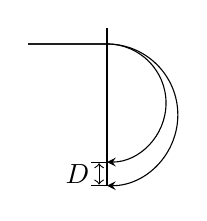
\begin{tikzpicture}
		\draw[-stealth] (0,0) -- (1,0) arc(90:-90:0.75cm); % (1,-1.5)
		\draw[-stealth] (0,0) -- (1,0) arc(90:-90:0.9cm);% (1,-1.8)
		\draw[|<->|] (0.9,-1.5) -- ++(0,-0.3)
			node[pos=0.5,left]{$D$};
		\draw (1,0.2) -- ++(0,-2);
	\end{tikzpicture}
\end{center}
\divisor

Poiché le velocità sono perpendicolari al campo magnetico le traiettorie sono archi di circonferenza
e la distanza $D$ non è altro che la differenza dei diametri. $D = 2(r_2-r_1)$.\\
Sugli ioni agisce la forza di Lorenz in quanto sono cariche in un campo magnetico. Dalla seconda legge
della dinamica possiamo dire che
\begin{equation*}
qvB = m\frac{v^2}{r}
\end{equation*}
Essendo la parte sinistra la forza di lorenz e quella destra nel caso in cui sia perpendicolare. Da
questa si deriva che
\begin{equation*}
r = \frac{mv}{qB}
\end{equation*}
La distanza è quindi pari a
\begin{equation*}
D = \frac{2v}{eB}(m_2-m_1) \approx \boxed{2.3\cdot10^{-3}\,\text{m}}
\end{equation*}

\paragraph{Esercizio 3}
Una barra conduttrice orizzontale di lunghezza $L$ e massa $m$ può scivolare su una guida verticale
(si guardi la figura) ed è in equilibrio ad un'altezza $L$ da un lungo cavo conduttore quando sia la
barra che il cavo hanno una corrente $I$ ma in versi opposti. \textbf{Trova $I$ in funzione di $L$ e
$m$. Qual è l'accelerazione iniziale della barra se la corrente del cavo venga improvvisamente
raddopiata?}
\begin{center}
	\begin{tikzpicture}
		\draw[thick] (0,0) -- (3,0);
		\draw[thick] (1,1) -- (2,1);
		\draw[dashed] (1,0.5) -- ++(0,2);
		\draw[dashed] (2,0.5) -- ++(0,2);
		
		\draw[|<->|] (0.8,1) -- ++(0,-1)
			node[pos=0.5,left]{$L$};
		\draw[|<->|] (1,0.8) -- ++(1,0)
			node[pos=0.5,below]{$L$};
		\node at (1.5,1.2){$\vec{i}$};
		\node at (1.5,-0.2){$-\vec{i}$};
	\end{tikzpicture}
\end{center}
\divisor

Abbiamo due fili paralleli attraversati da una corrente. Questo ci porta ad usare la legge di Ampére.
\begin{equation*}
F = \frac{\mu_0}{2\pi}\frac{i_1i_2}{d}l
\end{equation*}
Sostituendo i nostri dati otteniamo
\begin{equation*}
mg = \frac{\mu_0}{2\pi}\frac{-I^2}{\cancel{L}}\cancel{L}
\end{equation*}
Ora non resta che isolare $I$
\begin{equation*}
m=I^2\frac{\mu_0}{2\pi} \rightarrow \frac{2\pi m}{\mu_0}=I^2 \rightarrow 
\boxed{I = \sqrt{\frac{2\pi mg}{\mu_0}}}
\end{equation*}
Nel caso in cui la corrente si raddoppi, la forza raddoppia quindi diventa
\begin{equation*}
F=-I^2\frac{\mu_0}{\pi}=2mg
\end{equation*}
Usando la seconda legge di Newton ci dice
\begin{equation*}
F-mg=ma\rightarrow 2mg-mg = ma \rightarrow mg=ma
\end{equation*}
Questo ci dice che quindi $\boxed{a = g}$, verso l'alto.

\paragraph{Esercizio 4}
Un fascio di protoni con varie velocità è diretto nel verso positivo dell'asse $x$. Il fascio
entra in una regione in cui è presente un capo magnetico uniforme d'intensità $0.52\,\text{T}$;
il campo è diretto nel verso negativo dell'asse $z$, come indicato in figura.\\
Si vuole utilizzare un campo elettrico uniforme (in aggiunta al campo magnetico) per selezionare
solo quei protoni che hanno velocità pari a $1.42\cdot10^5\,\text{m/s}$; in altre parole si
vuole che questi protoni siano gli unici a non essere deflessi dai due campi.
\begin{enumerate}
  \item Determinare \textbf{l'intensità},  \textbf{la direzione} e \textbf{il verso} del campo
    elettrico che permette di selezionare le particelle
  \item Supponendo che il campo elettrico sia generato da un condensatore le cui amature distano
    $2.5\,\text{cm}$, calcolare la d.d.p.~necessaria da essere applicata agli estremi di esso
  \item Quale delle due armature deve essere caricata positivamente?
\end{enumerate}

\begin{center}
  \begin{tikzpicture}
    \tikzset{cross/.style={cross out, draw=black, minimum size=2*(#1-\pgflinewidth), 
      inner sep=0pt, outer sep=0pt},
      %default radius will be 1pt. 
      cross/.default={1pt}}
    \filldraw[gray] (0,0) -- ++(3,0) -- ++(0,-0.3) -- ++(-3,0) -- ++(0,0.3);
    \filldraw[gray] (0,-1.4) -- ++(3,0) -- ++(0,-0.3) -- ++(-3,0) -- ++(0,0.3);

    \foreach \y in {0.2, -0.5, -1.2, -1.9}{
      \foreach \x in {0,0.5,...,3}{
        \draw[thin] (\x,\y) circle (0.1);
        \draw[thin] (\x,\y) node[cross=2pt]{};
      }
    }

    \filldraw (-0.5,-0.8) circle (0.05);
    \draw[-stealth] (-0.5,-0.8) -- ++(0.3,0)
        node[pos=0.5,below]{$\vec{v}$};
  \end{tikzpicture}
\end{center}
\divisor

Abbiamo un campo magnetico e uno elettrico incrociati, questo è il tipico selettore di velocità.
La formula ci dice
\begin{equation*}
  v = \frac{E}{B}
\end{equation*}
e noi abbiamo $v$ e $B$. Il nostro compito quindi è ottenere $E$.
\begin{equation*}
  v = \frac{E}{B} \rightarrow E = vB = 1.42\cdot10^5\cdot0.52 = 
  \boxed{7.3\cdot10^4\,\text{C/m}^2}
\end{equation*}
In che direzione deve andare? Se osserviamo il campo magnetico generato, notiamo che tende a 
spingere i protoni verso l'alto (usando la regola della mano questo risulta evidente). Di
conseguenza, se si vuole mantenere stabile il protone, il campo elettrico deve andare verso
il basso, perpendicolarmente al condensatore.\\ [\baselineskip]
Un campo elettrico generato da un condensatore è pari a 
\begin{equation*}
  E = \frac{\Delta V}{\Delta x}
\end{equation*}
Noi abbiamo la distanza e il campo con la richieta della differenza di potenziale. Isoliamo
e calcoliamo
\begin{equation*}
  E = \frac{\Delta V}{\Delta x} \rightarrow \Delta V = E\Delta x = 7.3\cdot10^4\cdot0.025 = 
  \boxed{1846\,\text{V}}
\end{equation*}
Quale piastra deve essere caricata positivamente? Sapendo che il campo va da + a - e sapendo che
deve essere orientato verso il basso, la piastra positiva deve essere quella superiore.

\paragraph{Esercizio 5}
Un solenoide è lungo $20\,\text{cm}$ e ha un diametro di $50\,\text{mm}$. Il filo di rame 
utilizzato per formare le spire dell'avvolgimento ha una sezione di diametro $0.5\,\text{mm}$.
Le spire sono affiancate. Ai capi del solenoide è applicata una differenza di potenziale in
modo che il campo magnetico generato all'interno abbia un'intensità pari a $1.26\cdot10^{-3}\,
\text{T}$. La resistività del rame vale $1.7\cdot10^{-8}\,\Omega\cdot\text{m}$. \textbf{Calcola
il valore della differenza di potenziale.} 
\divisor

Scriviamo la formula che ci trova il campo magnetico in un solenoide
\begin{equation*}
  B = \mu_0 \frac{n}{l}i
\end{equation*}
La corrente è definita come
\begin{equation*}
  i = \frac{V}{R}
\end{equation*}
A noi manca anche la resistenza che però possiamo trovare facilmente usando la seconda legge di
Ohm
\begin{equation*}
  R = \rho \frac{L}{S} \rightarrow R = 1.7\cdot10^{-8} \frac{L}{\pi\cdot (2.5\cdot10^{-4})^2} =
  \underline{0.085L} 
\end{equation*}
Quindi ora, scrivendo tutto quanto in un'unica equazione
\begin{equation*}
  1.26\cdot10^{-3} = 4\cdot\pi \frac{n}{0.2}\frac{V}{0.085L}
\end{equation*}
dato che $L = 2n\cdot r\cdot\pi$ dato che il filo è arrotolato $n$ volte
\begin{equation*}
  1.26\cdot10^{-3} = 4\cdot\pi \frac{n}{0.2}\frac{V}{0.085\cdot n\cdot 0.15}
\end{equation*}
risolvendo per $V$ otteniamo
\begin{equation*}
  V = \boxed{2.67\,\text{V}}
\end{equation*}

\paragraph{Esercizio 6}
Un lungo filo metallico conduttore è piegato di $\ang{60}$ e si appoggia su un piano 
perpendicolare ad un campo magnetico uniforme $B_0 = 1\,\text{T}$. Un secondo filo metallico
molto lungo è tirato con una velocità $v=2\,\text{m/s}$ mentre si appoggia sul cavo piegato
in modo da formare un triangolo equilatero con i punti di contatto (si veda la figura). All'
istante $t=0$, il triangolo ha lato $l_0 = 0.5\,\text{m}$. Entrambi i cavi hanno una resistenza 
lineare unfirme di $\rho = 0.1\,\Omega\text{/m}$. Supponendo perfetto contatto tra i due cavi, si
esprima la forza elettromotrice indotta in funzione del tempo in termini di $B_0$, $v$, $l_0$ e 
$t$. \textbf{Qual è il valore di questa forza dopo $5\,\text{s}$? Trova la corrente in questo 
istante}.
\begin{center}
  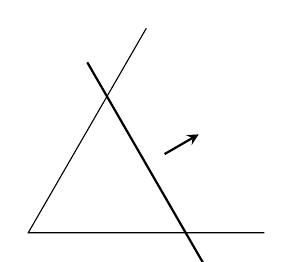
\begin{tikzpicture}
    \draw (3,0) -- (0,0) -- (60:3);
    \draw[thick, shorten <= -.5cm, shorten >= -.5cm] (2,0) -- (60:2);
    \draw[-stealth, thick] (30:2) -- (30:2.5);
  \end{tikzpicture}
\end{center}

\divisor

Ad un istante $t$, l'asta ha velocità $vt$ rispetto al piano della parte curva. Quindi la 
lunghezza del cavo che fa contatto è pari a
\begin{equation*}
  l = l_0 + 2vt\tan\ang{30} = l_0+\frac{2}{\sqrt{3}}vt
\end{equation*}
Man mano che si muove, il flusso continuerà a cambiare di intensità, quindi la forza 
elettromotrice continuerà a variare. Infatti
\begin{equation*}
  \mathcal{E} = B_0vl = B_0v \left( l_0+\frac{2}{\sqrt{3}}vt \right)
\end{equation*}
A $t=5$, basta soltanto sostituire per ottenere
\begin{equation*}
  \mathcal{E} = B_0v \left( l_0+\frac{2}{\sqrt{3}}vt \right) \rightarrow 1\cdot2 
  \left[ 0.5+\left( \frac{2}{\sqrt{3}} \right)\cdot 2\cdot5 \right] = \boxed{24.1\,\text{V}}
\end{equation*}
La resistenza del filo è costante ed è pari a $R = 3l\rho$ perché consideriamo tutto il circuito
chiuso. Vediamo che la resistenza è dipendente dal tempo (per la presenza del fattore $l$).
Di conseguenza la corrente non è altro che
\begin{equation*}
  i = \frac{\mathcal{E}}{R} = \frac{B_0v\cancel{l}}{3\cancel{l}\rho} \rightarrow 
  i = \boxed{6.67\,\text{A}}
\end{equation*}
